\section{Evaluation}
\label{sec:evaluation}
%% \jrex{start with a brief roadmap of the section.}

We now evaluate \TheSystem through trace-driven simulations. We tune the
main parameter of \TheSystem---the number of table stages $d$---in
\Sec{subsec:sensitivity}. We evaluate the performance of \TheSystem in isolation
in \Sec{subsec:isolatedEvaluation}, and then compare it to prior sampling and
sketching solutions in \Sec{subsec:comparisonRelated}. Then, we examine the
performance of \TheSystem in context of the idealized algorithms it is derived from
(\Sec{sec:algorithm}) in \Sec{subsec:comparisonIdeal}.

\NewPara{Experiment setup.} We compute the $k$ heaviest flows using two sets of
traces. The first trace is from a 10Gb/s ISP backbone link, recorded in 2016 and
available from CAIDA~\cite{caida}. We measure heavy hitters aggregated by
transport 5-tuple.
The traffic trace is 17 minutes long, and
contains 400 million packets. We split this trace into 50 chunks, each being
about 20 seconds long, with 10 million packets. The chunks on average
contain about 400,000 5-tuple flows each. Each chunk is one trial, and each data
point in the graphs for the ISP trace reports the average across 50 trials. We
assume that the switch zeroes out its tables at the end of each trial, which
corresponds to a 20 second ``table flush'' period. %% It is feasible to flush the
%% table this often in switch hardware; switches can already rewrite tables at
%% intervals of tens of seconds or smaller, \eg~\cite{bgp-neighbor-timer,
%%   netflow-timer, li2016flowradar}.

The second trace, recorded in 2010, is from a data center~\cite{theo-dc-traffic}
and consists of about 100 million packets in total. We measure heavy hitters
aggregated by source and destination IPs. We split the trace into 1 second
intervals corresponding to the time scale at which data center traffic exhibits
stability~\cite{microTE}.

The data center trace is two and a half hours long, with roughly 10K packets
(300 flows) per 
second. We additionally replay the trace at two higher packet rates to test
whether \TheSystem can provide good accuracy over the 1 second time scale. We
assume a ``typical'' average packet size of 850 bytes and a 30\% network
utilization as reported in prior traffic studies~\cite{theo-dc-traffic}. For a
switch clocked at 1GHz with 48 ports of 10Gb/s each, this corresponds to roughly
20 million packets per second through the entire switch, and 410K packets per
second through a single link. At these packet rates, the trace contains
20,000 and 3200 flows per second respectively. For each packet rate, we report
results averaged
from multiple trials of 1 second each.

%% The results we report are averaged from multiple
%% samples corresponding to 1 second chunks of the trace corresponding to the three
%% different packet rates.

%% Given that the traffic is relatively stable over 1 -
%% 2s intervals, we chunk the trace accordingly. This results in about 10K packets
%% per second. We also "fast-forward" the traces to the single switch rate of about
%% 20 million packets per second and the single link rate of 410 million packets
%% per second. Once the origincal trace is chunked accordingly, we treat each chunk
%% as one trial and each data point in the following graphs reports the average
%% across all trials.

\NewPara{Metrics.} As discussed in \Sec{sec:problem}, we evaluate schemes on
false negatives (\% heavy flows that are not reported), false positives (\%
non-heavy flows that are reported), and the count estimation error (\% error for
heavy flows). Note that for the top-$k$ problem, the false positive error is
just a scaled version of the false negative.

\subsection{Tuning \TheSystem}
\label{subsec:sensitivity}

Given a total memory size $m$, \TheSystem's only tunable parameter is the number
of table stages $d$ that it uses. Once $d$ is fixed, we simply partition the
available memory equally into $d$ hash tables. As $d$ increases, the number of
table slots over which a minimum is computed increases, leading to increased
retention of heavier keys. However, with a fixed total memory, an increase in
the value of $d$ decreases the per-stage hash table size, increasing the
likelihood of hash collisions, and also of duplicates
(\Sec{sec:feed-forward}). The switch hardware constrains the number of table
stages to a small number, \eg 6-16~\cite{intel-fm6000, RMT}.

\Fig{falseNegvsD} shows the impact of changing $d$ on the false negatives. For
the ISP trace, we plot false negatives for different sizes of memory $m$ and
different number of desired heavy hitters $k$. As expected, the false negatives
reduce as $d$ increases starting at $d=2$, but the decrease quickly tapers off
in the range between 5--8, across the different $(m,k)$ curves. For the data
center trace, we show false negatives for $k=350$ with a memory of 840 counters
(15KB), and we see a similar trend across all three packet rates. The false
positives, elided here, also follow the same trend.

To understand whether duplicates impact the false negative rates, we also show
the prevalence of duplicates in \TheSystem's hash tables in
\Fig{duplicates}. Overall, duplicates only take up between 5-10\% of the
available table size in the ISP case and between 5-14\% in the data center
case. As expected, in going from $d=2$ and $d=8$, the prevalence of duplicates
in \TheSystem's table increases.

\Fig{estimation-error-D} shows the count estimation error (as a
percentage of actual flow size) {\em for flows in
  \TheSystem's tables} at the end of each measurement interval, with a memory
size of 640 counters (11.2KB).
%
In general, the
error reduces as $d$ increases, but the reduction from $d=4$ to $d=8$ is less
significant than the reduction from $d=2$ to $d=4$.
%
In the ISP trace, the estimation error is stable across flow sizes since most
flows recorded by \TheSystem have sizes of at least 1000.
%
In the data center trace where there are fewer total flows, there is a more
apparent decrease in error with true flow size, with flows of size $x > 1000$
having near-perfect count estimations.

\NewPara{Choosing $d=6$ table stages.} To summarize, we find that (i) as the
number of table stages increases above $d=4$, all the accuracy metrics improve;
(ii) however, the improvement dimishes at $d=8$ and beyond, due to the increasing
prevalence of duplicates and hash collisions. These trends hold across both the
ISP and data center scenarios, for a variety of measured heavy hitters $k$ and
memory sizes. Hence, we choose $d=6$ table stages for all further experiments
with \TheSystem.

%% \iffalse
%% \begin{figure}[h]
%% \includegraphics[max height=11cm,max width=8cm]{WFalseNegsvsDsSingle.pdf}
%% \caption{Weighted fraction of Heavy Hitters Reported for Different $d$ values  with 500000 flows in total}
%% \label{fig:weightedNegvsD}
%% \end{figure}
%% \fi

\begin{figure}
  \centering
  \[
  \begin{array}{ccc}
	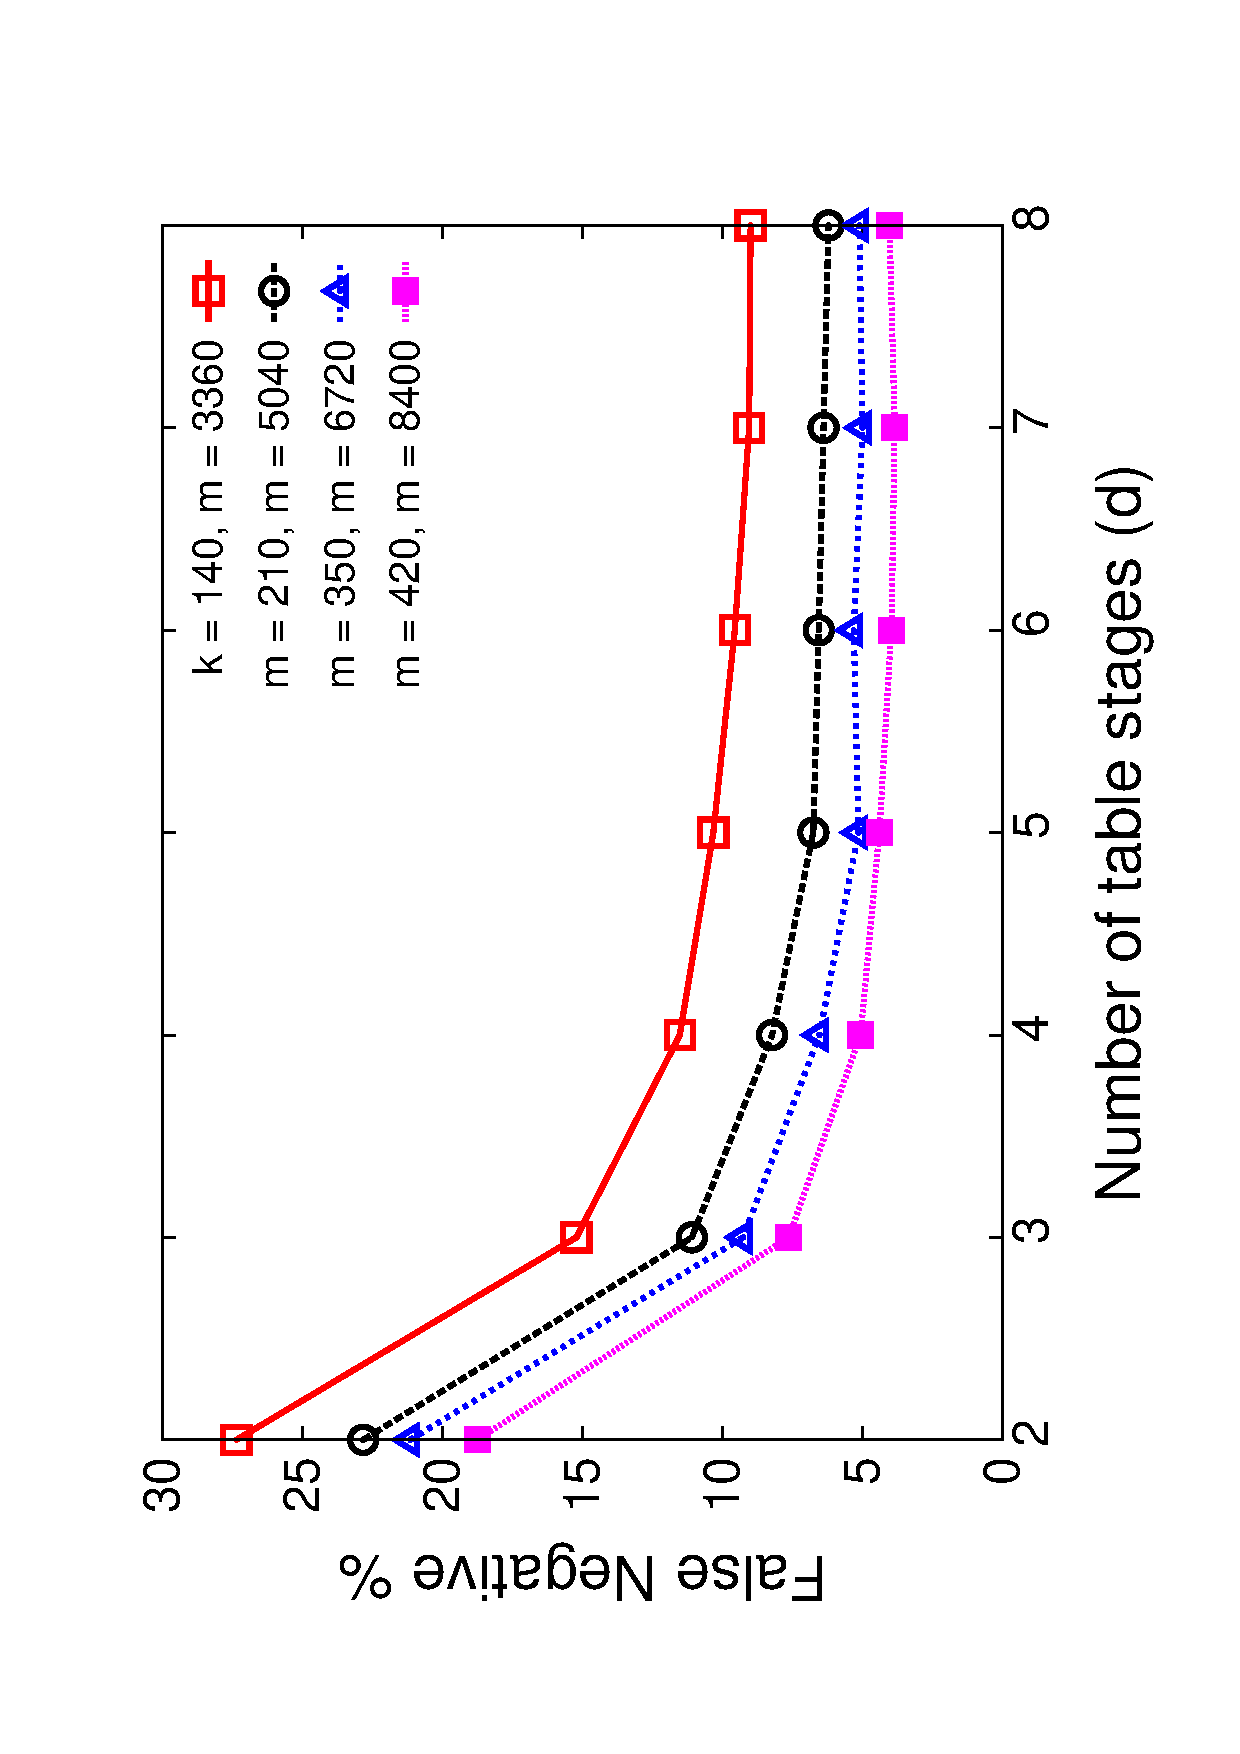
\includegraphics[width=.49\columnwidth]{FalseNegvsDSingle.pdf} &
	\includegraphics[width=.49\columnwidth]{FalseNegvsDTheo.pdf}
    \\
    \mbox{(a) ISP backbone} & \mbox{(b) Data center} \\
  \end{array}
  \]
\caption{Impact of table stages ($d$) on false negatives. Error
  decreases as $d$ grows, and then flattens out.}
\label{fig:falseNegvsD}
\end{figure}

%% \iffalse
%% \begin{figure}[h]
%% 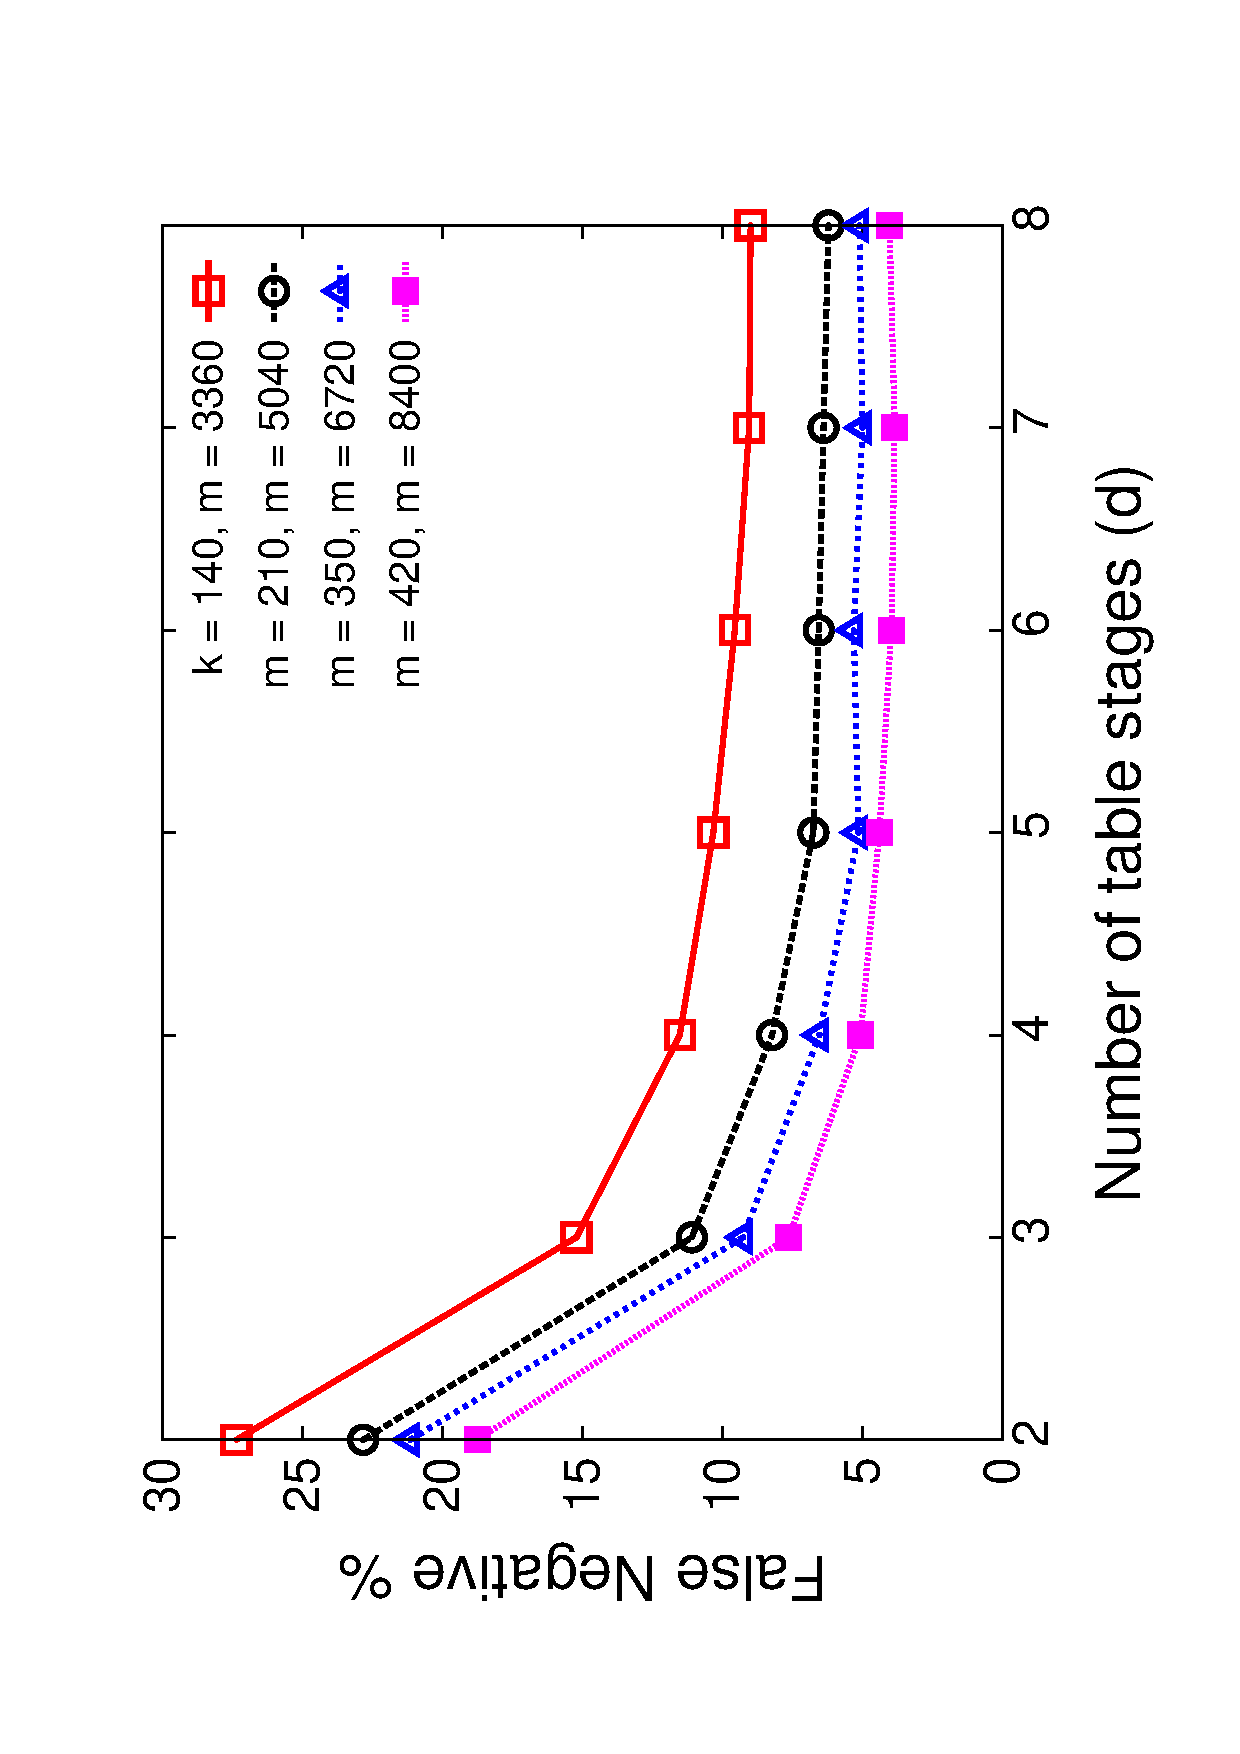
\includegraphics[max height=11cm,max width=8cm]{FalseNegvsDSingle.pdf}
%% \caption{Impact of the number of table stages on false negatives. Error
%%   decreases as $d$ grows, and then flattens out.}
%% \label{fig:falseNegvsD}
%% \end{figure}
%% \fi

\begin{figure}
  \centering
  \[
  \begin{array}{ccc}
	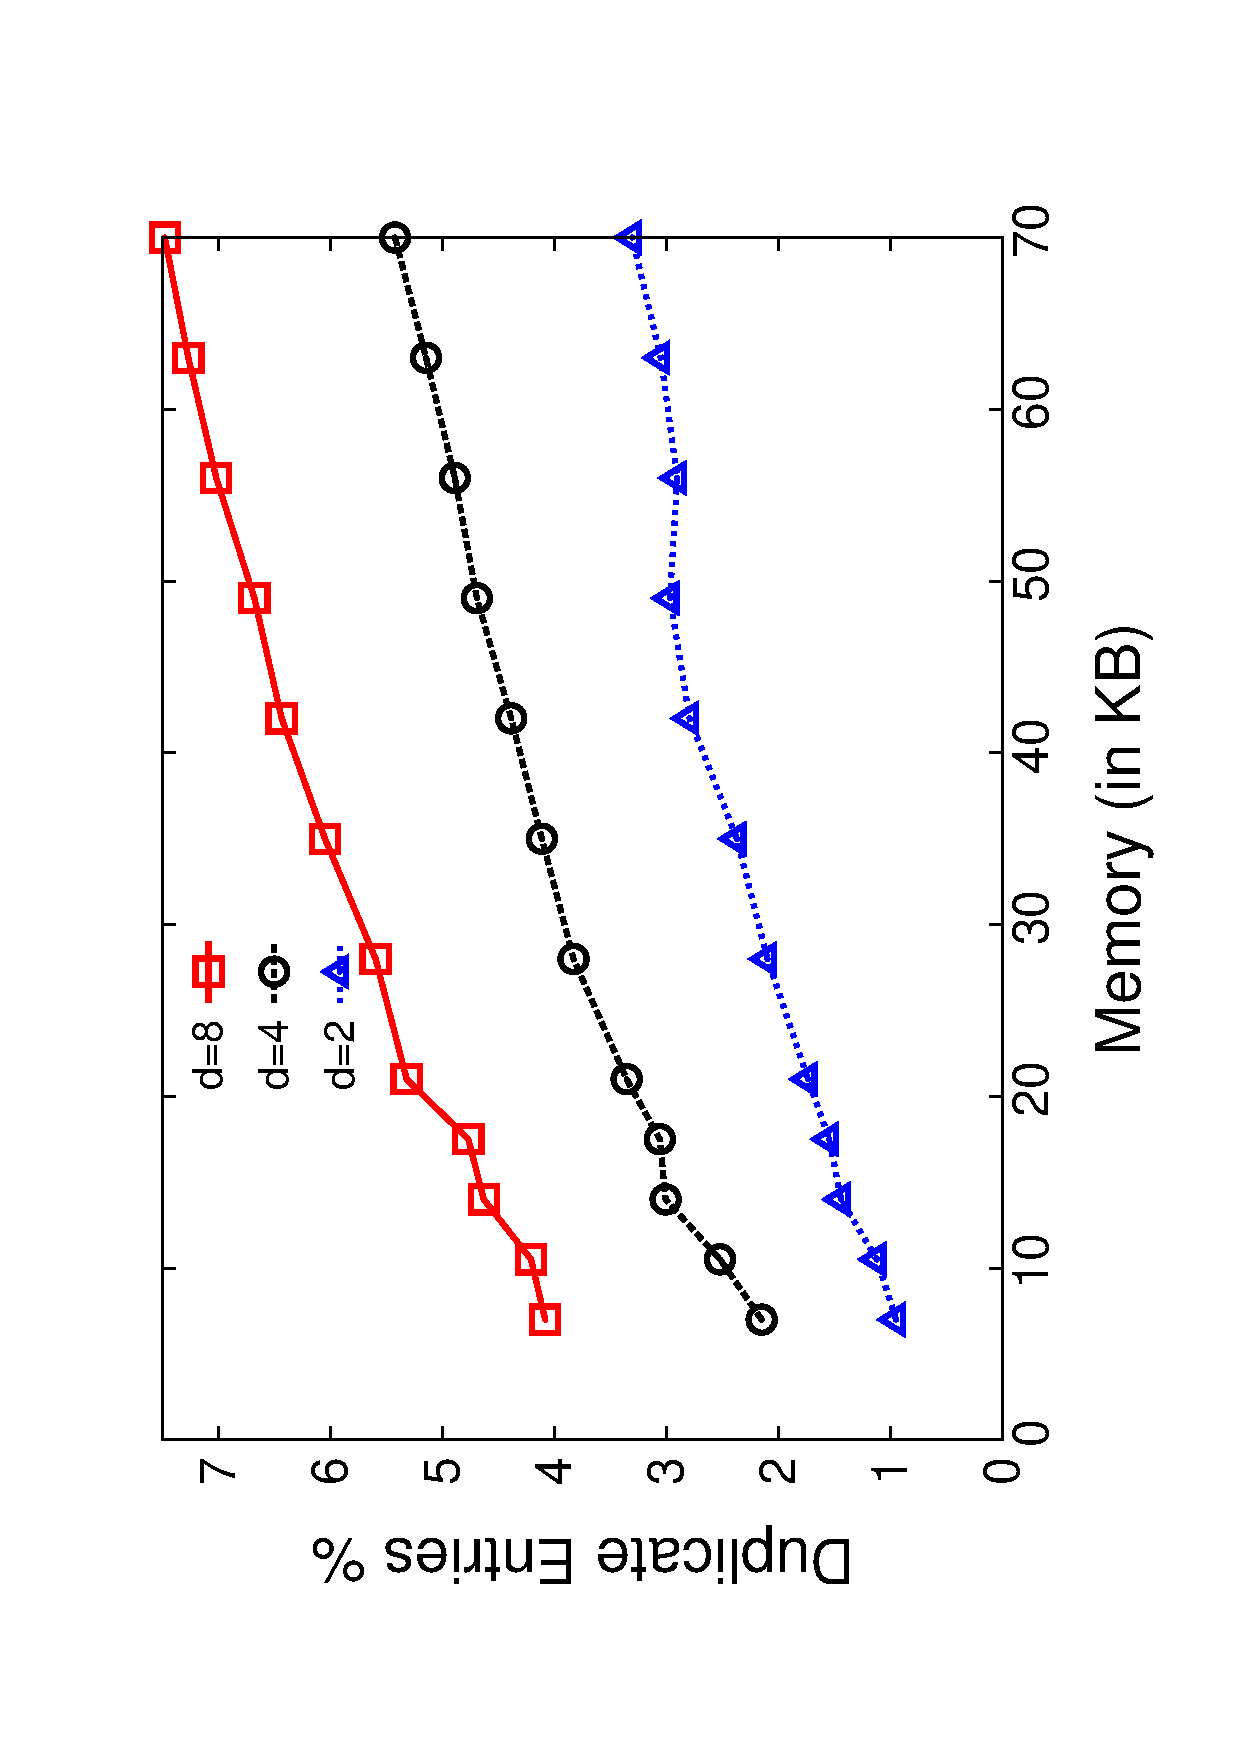
\includegraphics[width=.49\columnwidth]{Duplicates.pdf} &
	\includegraphics[width=.49\columnwidth]{TheoDuplicates.pdf}
    \\
    \mbox{(a) ISP backbone} & \mbox{(b) Data center (link)} \\
  \end{array}
  \]
\caption{Prevalence of duplicate keys in tables. For different $d$ values under
  the memory range tested, the proportion of duplicates is between 5-10\% for
  the ISP trace and 5-15\% for the data center trace (link packet rate).}
\label{fig:duplicates}
\end{figure}

%% \iffalse
%% \begin{figure}[h]
%% 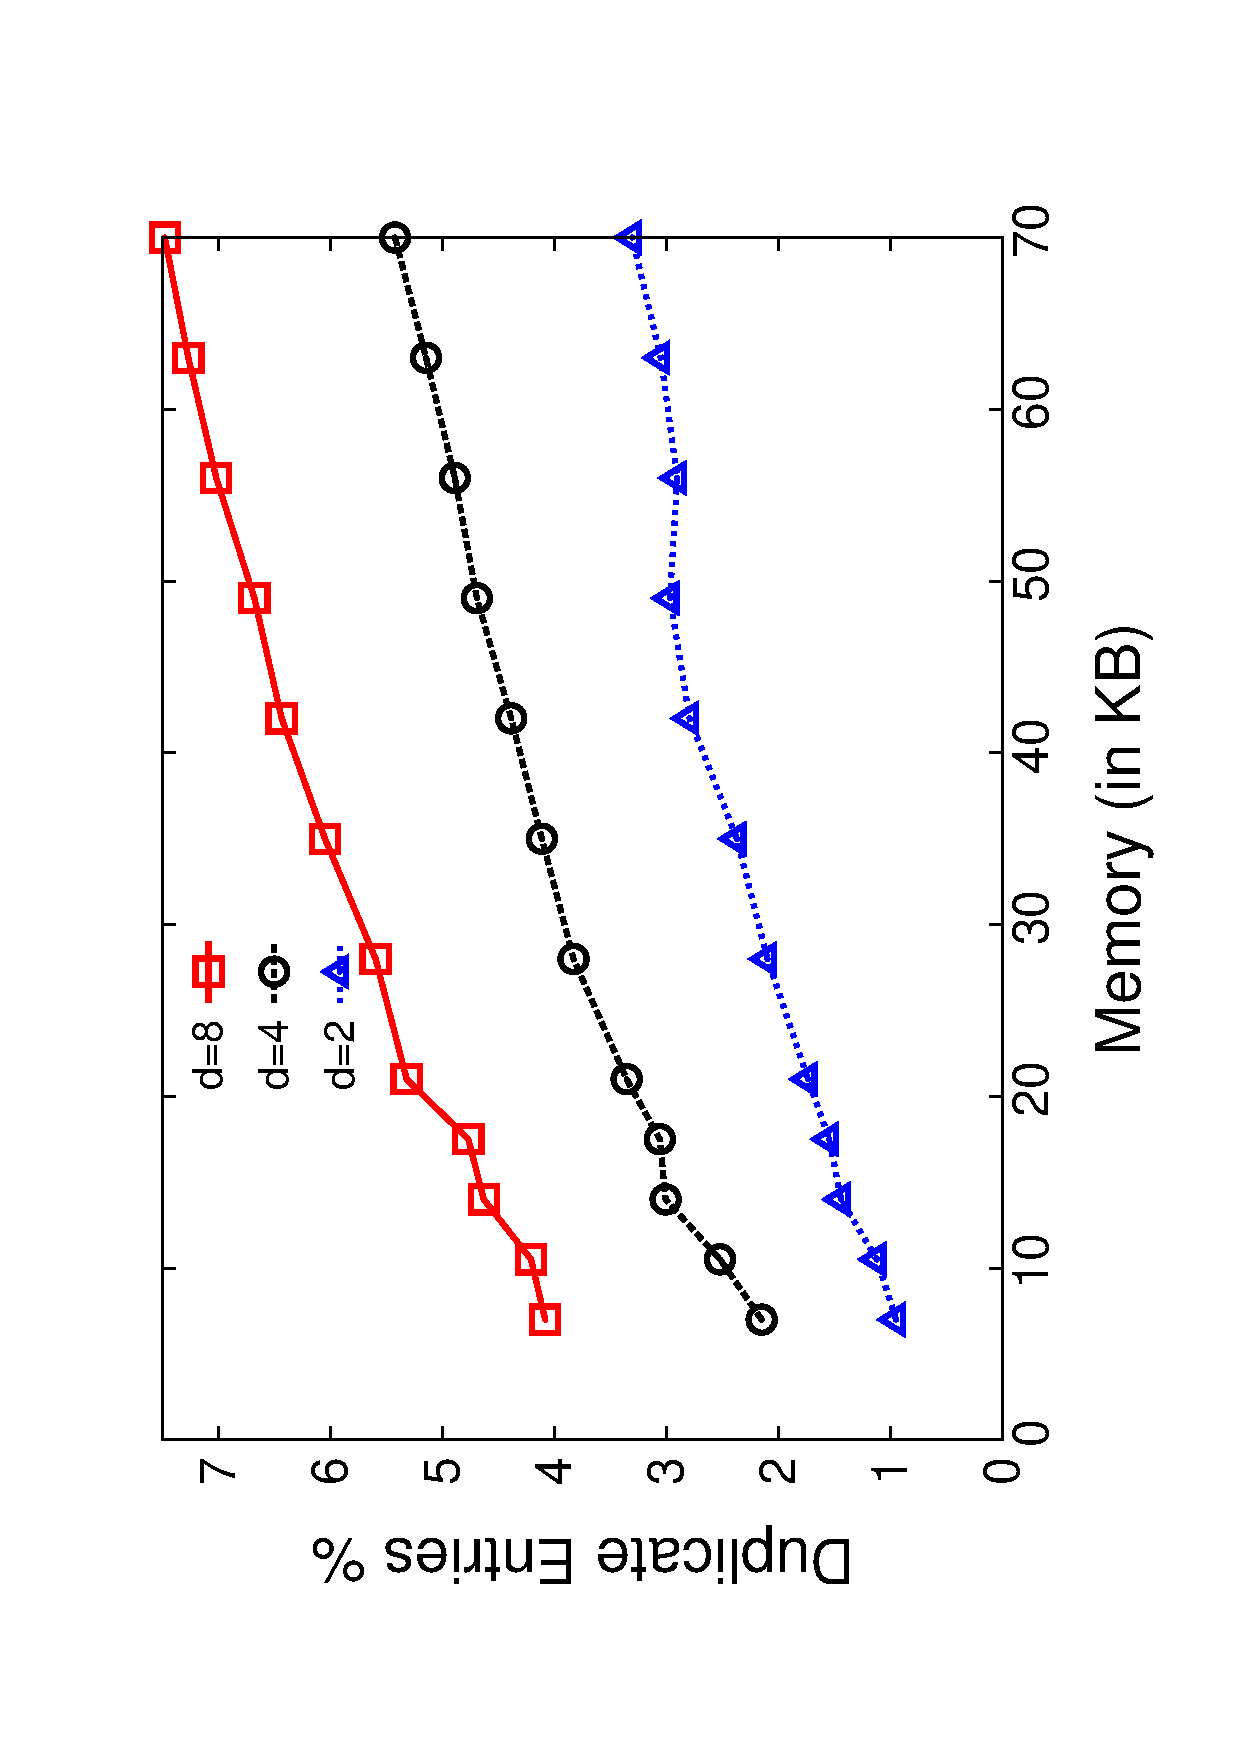
\includegraphics[max height=11cm,max width=8cm]{Duplicates.pdf}
%% \caption{Prevalence of duplicate keys in \TheSystem's tables.}
%% \label{fig:duplicates}
%% \end{figure}
%% \fi


%% \begin{figure}
%%   \centering
%%   \[
%%   \begin{array}{ccc}
%% 	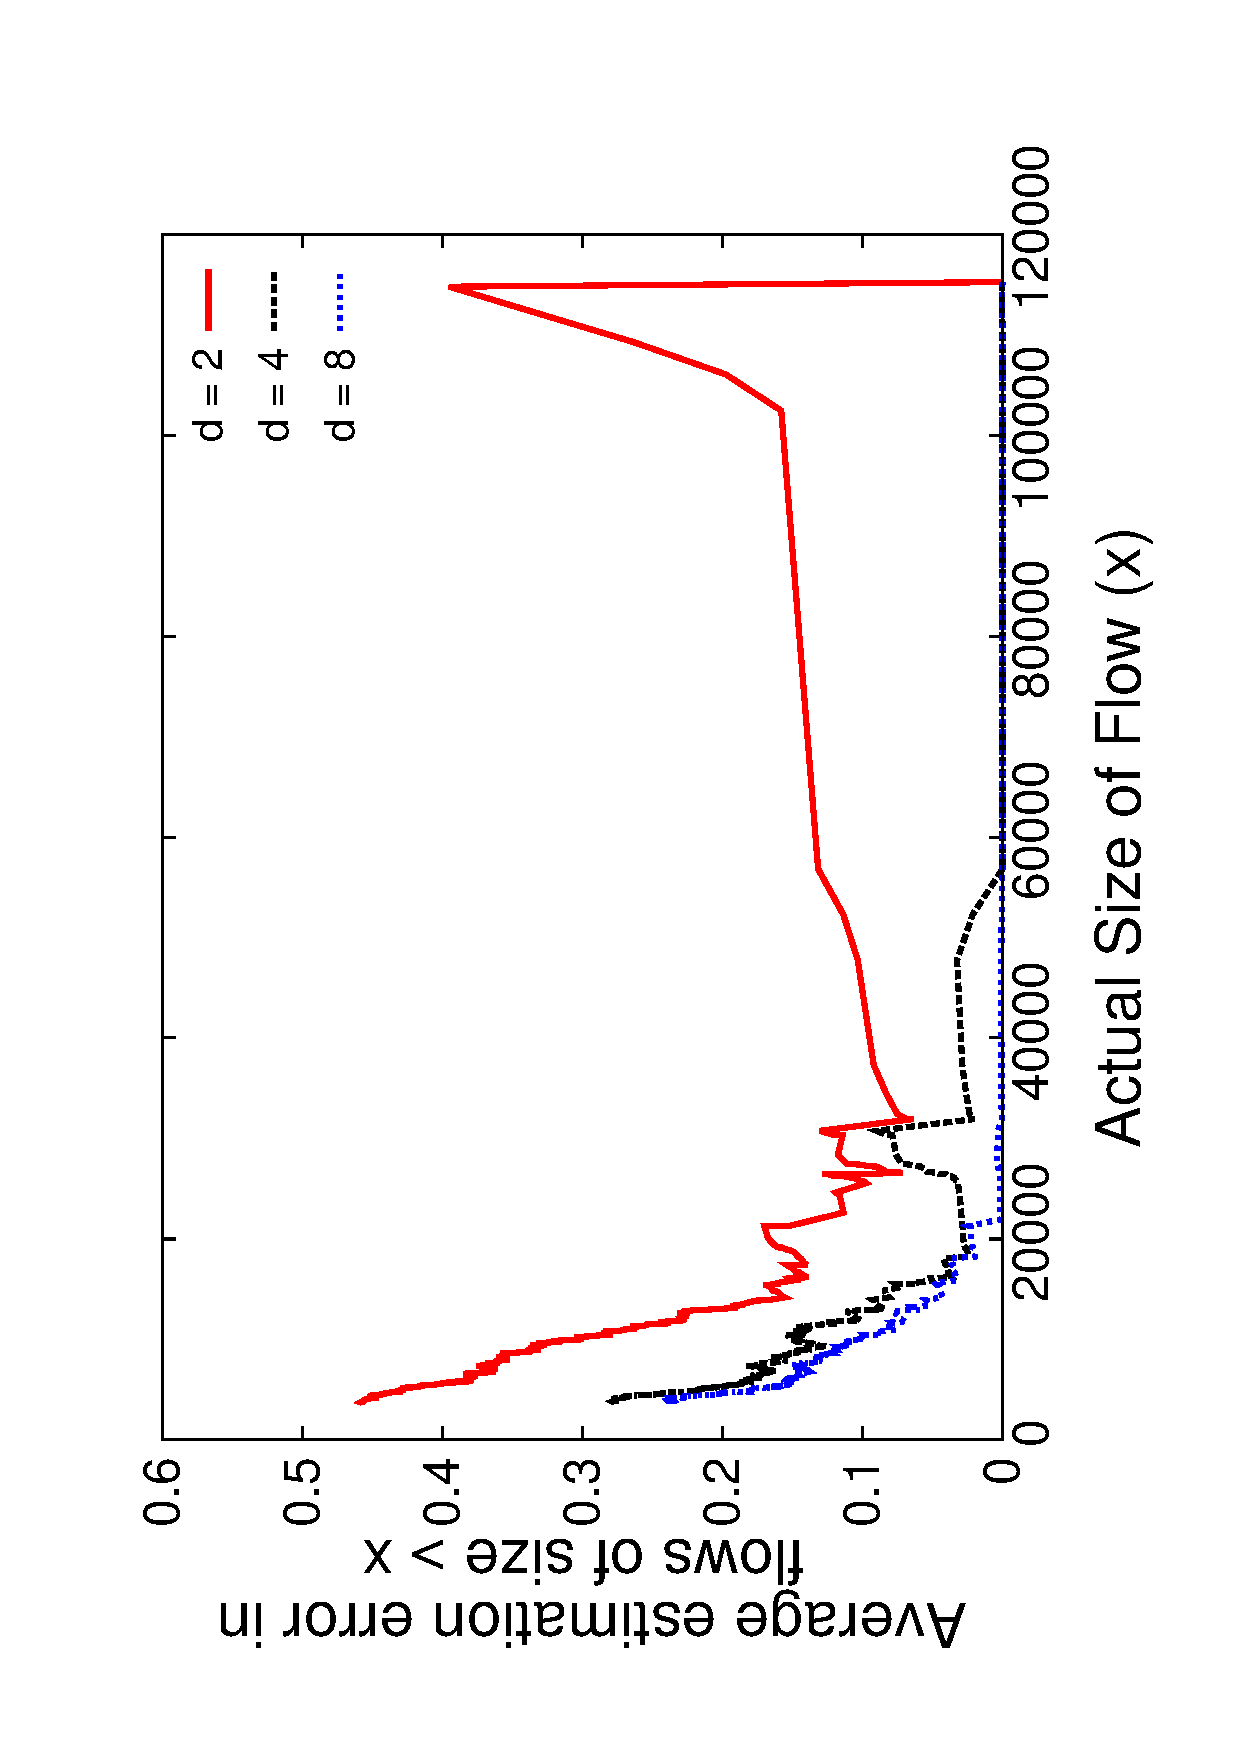
\includegraphics[width=.49\columnwidth]{DsRelativeError.pdf} &
%% 	\includegraphics[width=.49\columnwidth]{TheoDsRelativeError.pdf}
%%     \\
%%     \mbox{(a)} & \mbox{(b)} \\
%%   \end{array}
%%   \]
%% \caption{Comparison of average estimation error (\%) of flows whose true counts   are higher than the $x$-value in the graph. Error
%%  decreases as $d$ grows, yet, the difference is less pronounced at higher $d$. (a) CAIDA Trace (b) Data Center packet rate for a single link}
%% \label{fig:estimation-error-D}
%% \end{figure}

\begin{figure}
  \centering
  \[
  \begin{array}{ccc}
	\includegraphics[width=.49\columnwidth]{DsRelativeErrorAlt.pdf} &
	\includegraphics[width=.49\columnwidth]{TheoDsRelativeErrorAlt.pdf}
    \\
    \mbox{(a) ISP backbone} & \mbox{(b) Data center (link)} \\
  \end{array}
  \]
\caption{Average estimation error (\%) of flows whose true counts are higher
  than the $x$-value in the graph. Error decreases as $d$ grows but the benefit
  diminishes with increasing $d$. Error decreases with actual flow size.}
\label{fig:estimation-error-D}
\end{figure}

%\begin{figure}[h]
%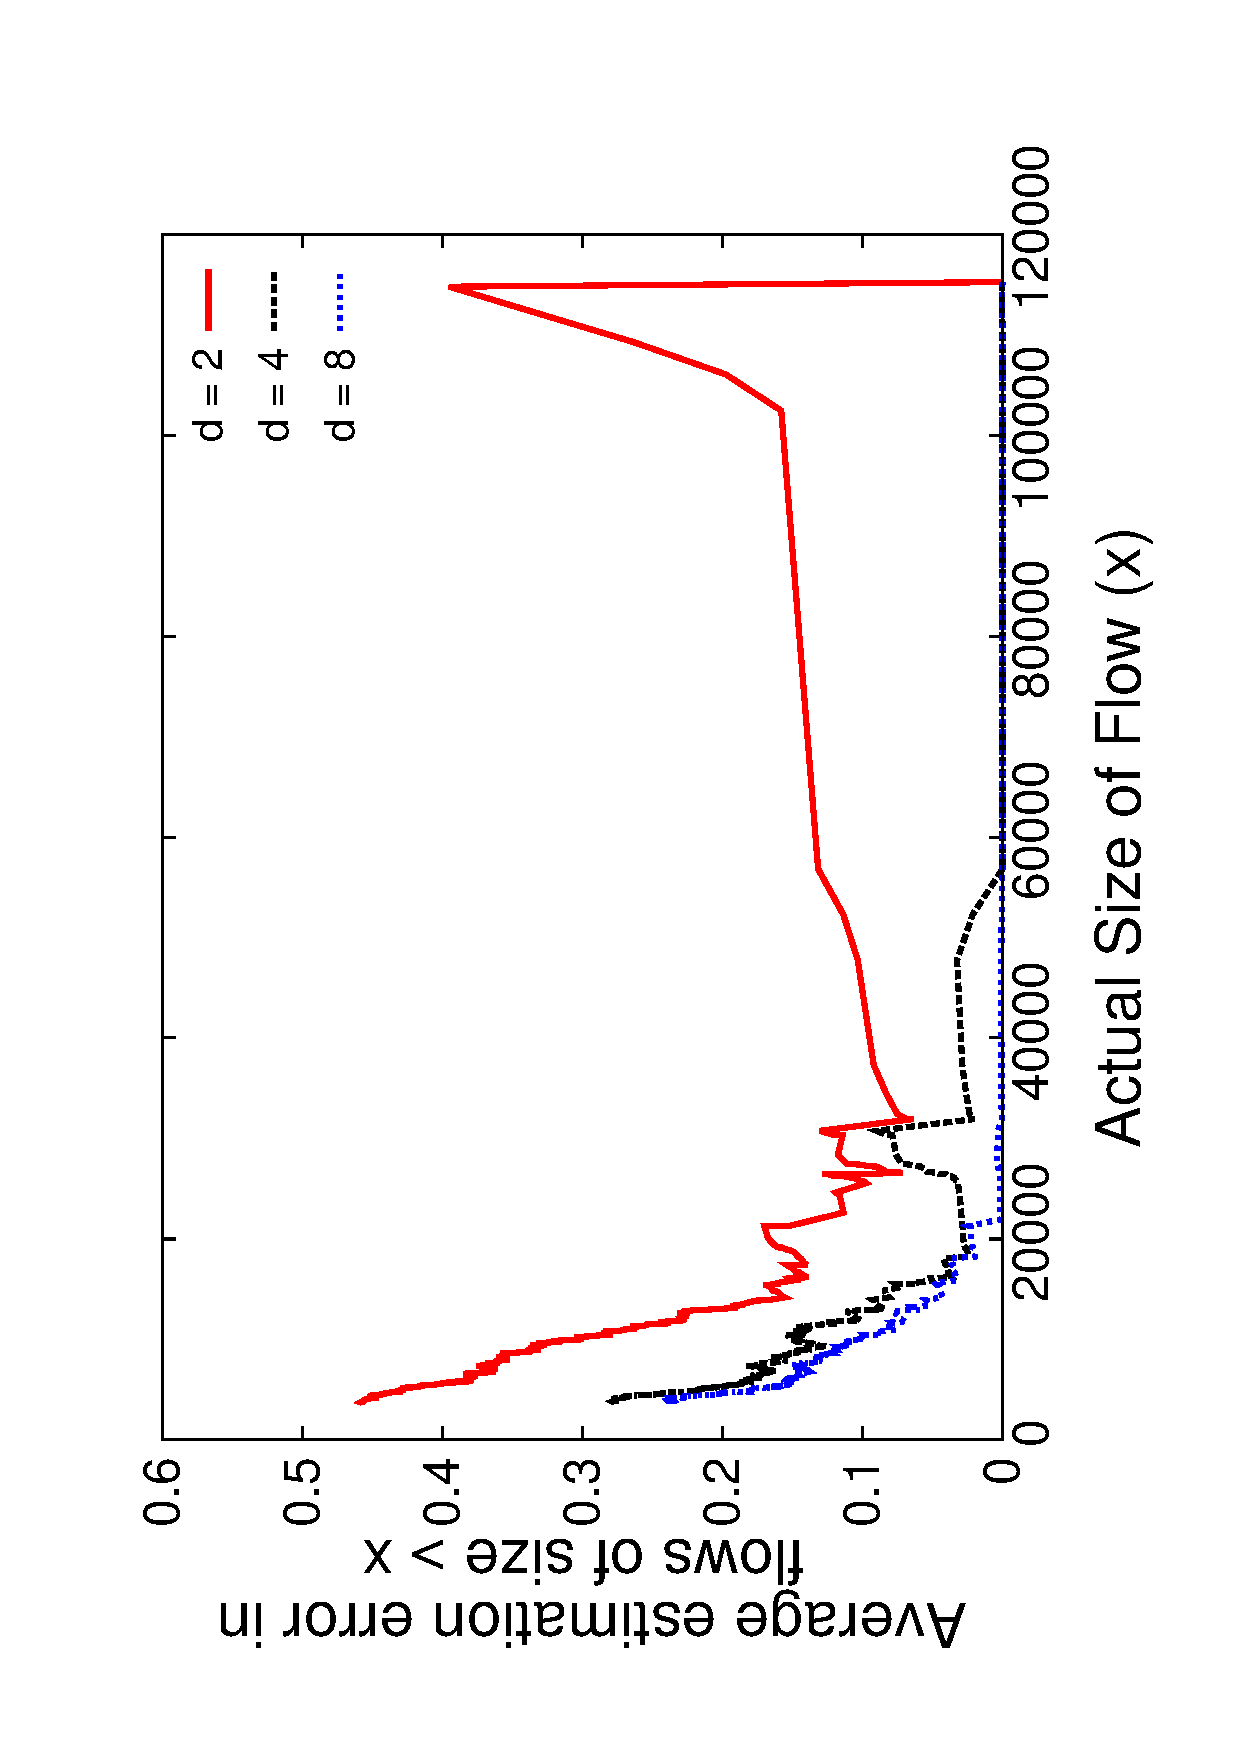
\includegraphics[max height=11cm,max width=8cm]{DsRelativeError.pdf}
%\caption{Comparison of average estimation error (\%) of flows whose true counts
%  are higher than the $x$-value in the graph. Error
% decreases as $d$ grows, yet, the difference is less pronounced at higher $d$}
%\label{fig:estimation-error-D}
%\end{figure}

%% In order to enure that the algorithm preserves the feed-forward property,
%% \TheSystem always inserts the incoming flow in stage $1$ an then computes the
%% minimum in a rolling fashion (\Sec{sec:feed-forward}). However, this could
%% induce some duplicates in the table when a flow present in a later table
%% stage is inserted afresh in the first table stage. Figure
%% \ref{fig:duplicates} shows that the fraction of the table occupied by
%% duplicates increases as the memory provisioned is increased but that this is
%% a small fraction (around $5\%$) of the total memory available for
%% heavy-hitter detection. %smaller memories, fewer %duplicates - get evicted
%% (or coalesced) for %larger flows - shows up as underestimates?


\subsection{Accuracy of \TheSystem}
\label{subsec:isolatedEvaluation}

We plot error \vs memory tradeoff curves for \TheSystem, run with $d=6$ table
stages. Henceforth, unless mentioned otherwise, we run the data center trace at
the single link packet rate.

\NewPara{False negatives.} \Fig{HPNegvsM} shows the false negatives as memory
increases, with curves corresponding to different numbers of reported heavy
hitters $k$. We find that error decreases with allocated memory across a range
of $k$ values, and settles to under 10\% in all cases on the ISP trace at 80KB
of memory, which corresponds to 4500 counters. 
%
In any one trial with the ISP trace, there are on average 400,000 flows, which
is two orders of magnitude higher than the number of counters we use.
%
In the data center trace, the error settles to under 10\% at just 9KB of memory
(520 counters) for all the $k$ values we tested.\footnote{The minimum memory
  required at $k=300$ is 6KB ($\approx$ 300 counters).}

These results also enable us to understand the interplay between $k$ and the
memory size required for a specific accuracy. For a 5\% false negative rate in the
ISP trace, the memory required for $k=60$ is 60KB ($3375 \approx 55k$ counters),
whereas the memory required for $k=300$ is 110KB ($6200 \approx 20k$ counters).
%% At 110KB memory ($m=6200$
%% counters) for the ISP trace, we find that the error is about 5\% for $k=300$
%% ($m \approx 20k$), and around 2\% for $k=60$ ($m \approx 100k$). 
%
%% For $k=300$, the error drops under 10\% at about 4000 counters ($\sim 13k$)
%% counters, and for $k=60$ around 2000 counters ($\sim 33k$).
%% (As memory increases beyond the range shown, false negatives continue to
%%drop.)
%% Recall that there are about 400,000 flows on average in any one trial in this trace, which is two orders of magnitude higher than the number of counters used here.
In general, the factor of $k$ required in the number of counters to
achieve a particular accuracy reduces as $k$ increases.

%% We also evaluate the memory-accuracy tradeoff for \TheSystem when one is
%% interested in the top-$k$ flows. Figure \ref{fig:HPNegvsM} and \Fig{HPPosvsM}
%% captures this tradeoff for different values of $k$. The trend indicates, as
%% expected, that for a given $k$ value, the accuracy improves as we provision more
%% memory. Given that the individual $20s$ traces contain around $0.5M$ flows by
%% 5-tuple on average, we are able to detect on the order of $100$ heavy flows
%% amongst the $0.5M$ with less than $10\%$ false negatives using less than $5K$
%% entries or $80 KB$ of space! This translates to needing roughly $15-20$ times
%% $k$ entries to track the top-$k$ heavy hitters to achieve a false negative rate
%% that is lower than $10\%$. At even higher memory, the false negative rate drops
%% to $5\%$. The exact factor is different across different $k$. As you increase
%% $k$, the curves start dropping faster. For example, at $k=60$, $1500$ or $25x$
%% entries are needed, while at $k=240$, less than $4500$ or $18$x entires are
%% needed.

%% \iffalse
%% \begin{figure}[ht]
%% 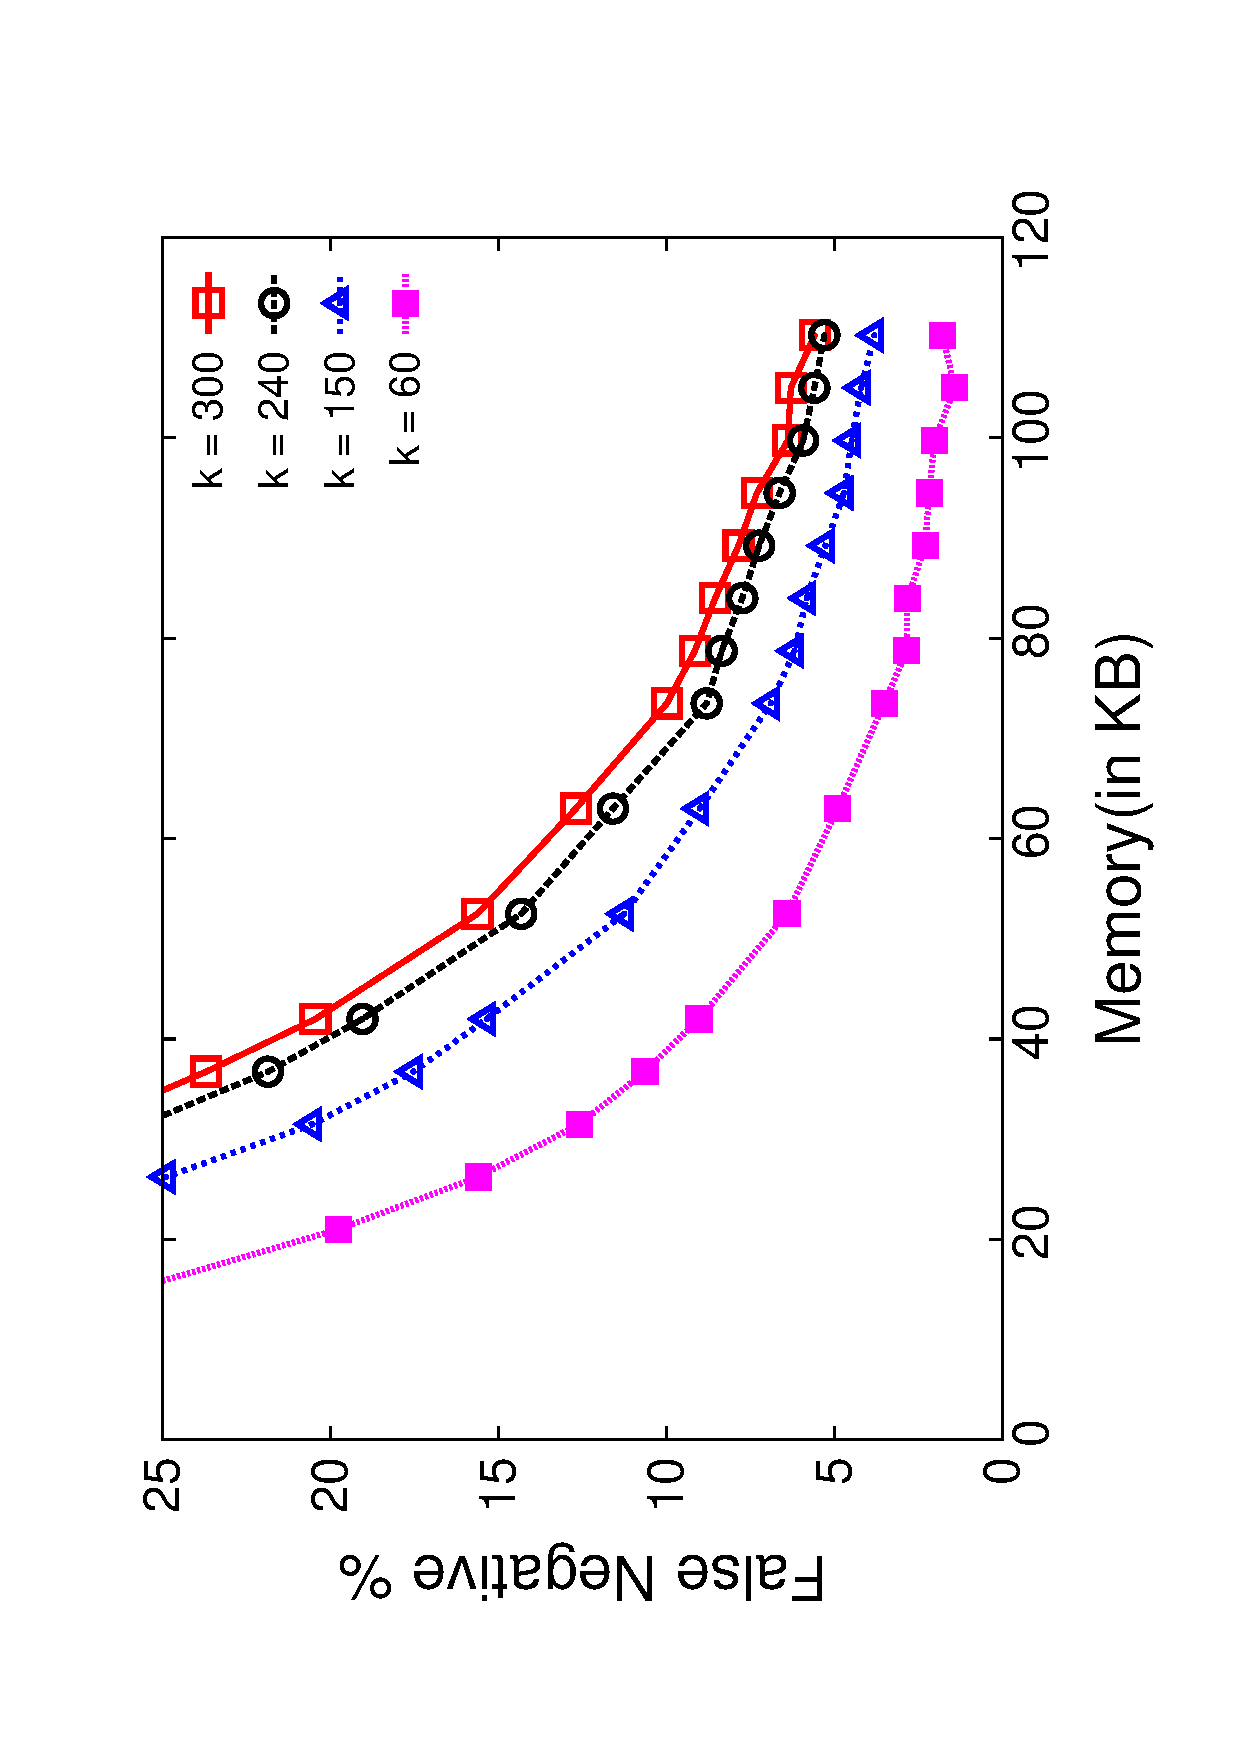
\includegraphics[width=\columnwidth]{FalseNegsvsMsSingle.pdf} % previously [width=0.45\columnwidth]
%% \caption{False negatives of \TheSystem with increasing memory. Each trial trace
%%   contains an average of 400,000 flows, but \TheSystem achieves between 5-10\%
%%   false negatives for the top 60-300 heavy hitters with just 4500 flow
%%   counters.}
%%   %% Accuracy of reported Heavy hitters for Different $m$ values at $d = 6$ with
%%   %% $0.5M$ flows. $80KB$ translates to about 4500 key, value pairs
%% \label{fig:HPNegvsM}
%% \end{figure}
%% \fi

\begin{figure}
  \centering
  \[
  \begin{array}{ccc}
	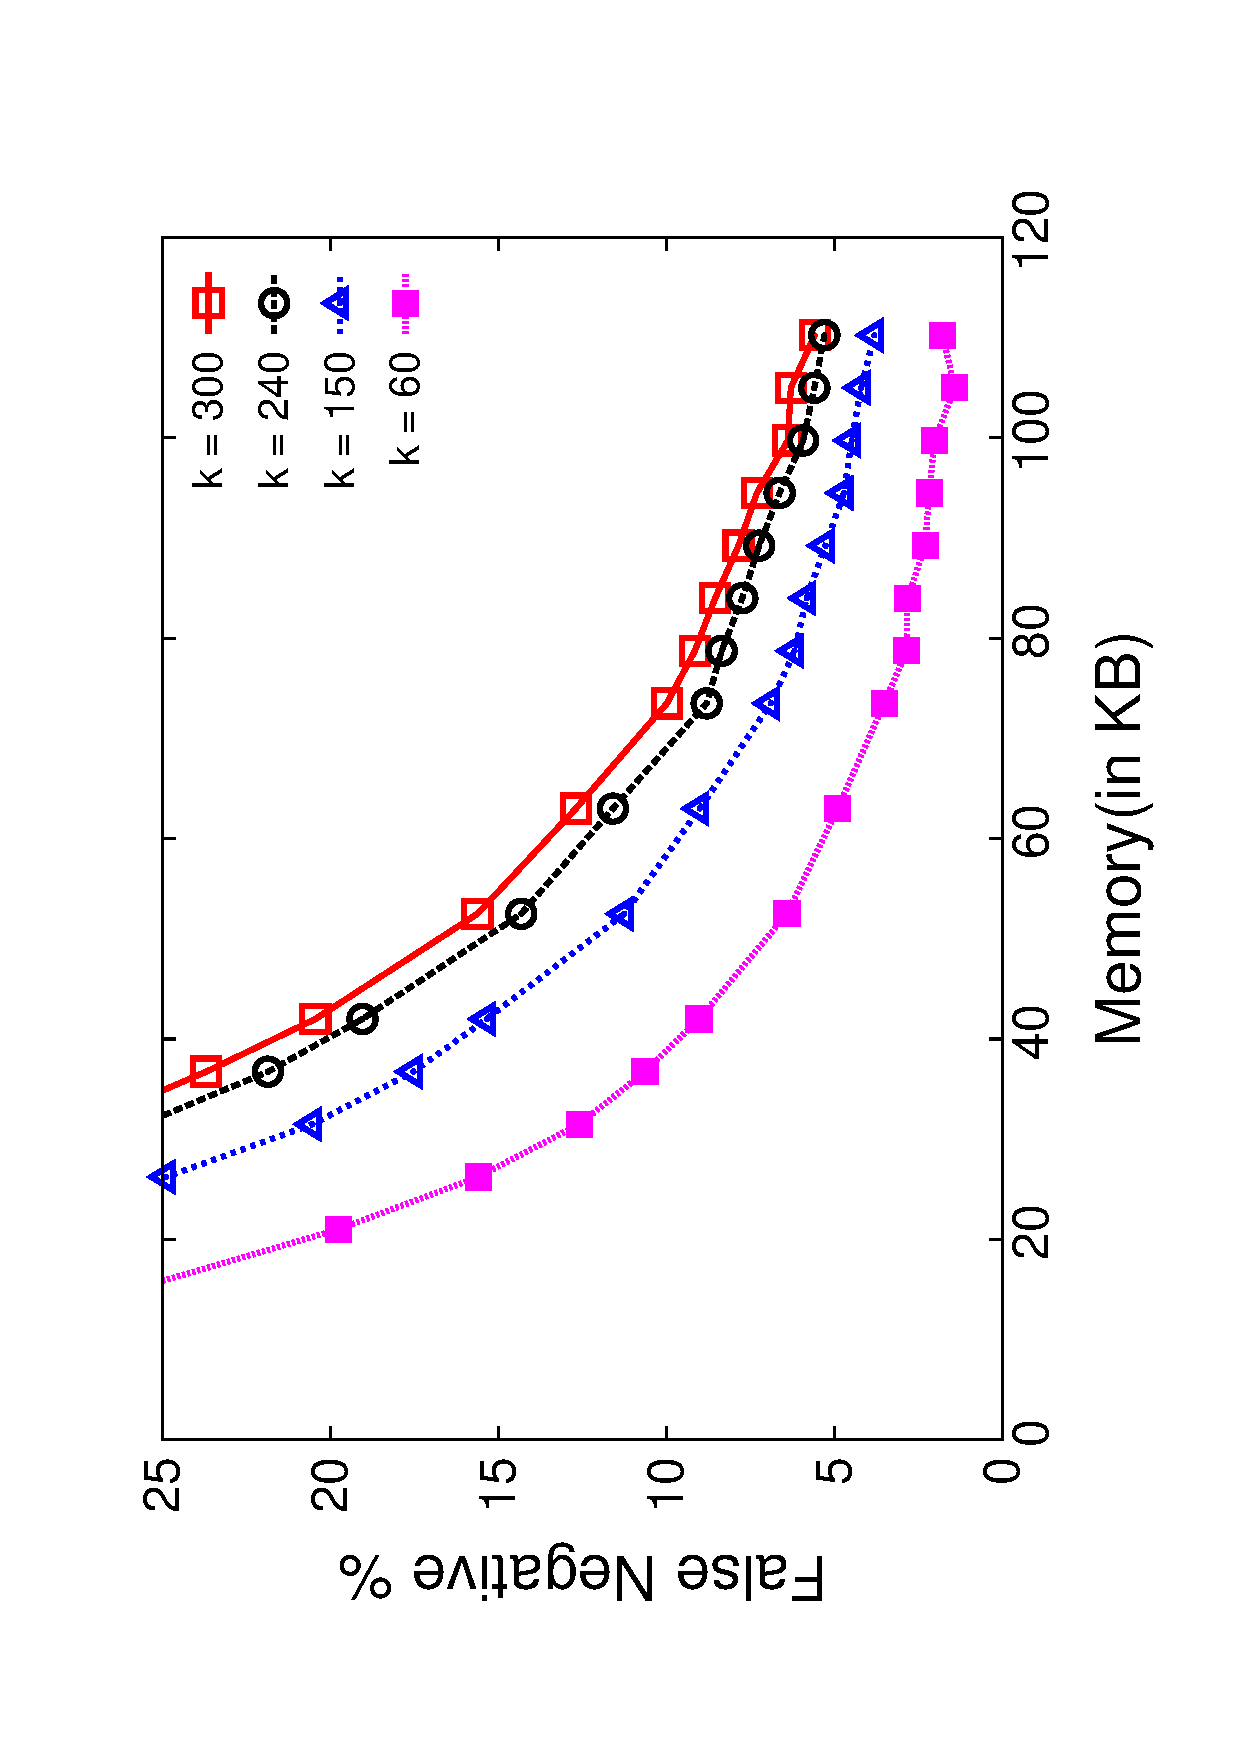
\includegraphics[width=.49\columnwidth]{FalseNegsvsMsSingle.pdf} &
	\includegraphics[width=.49\columnwidth]{FalseNegsvsMsTheo.pdf}
    \\
    \mbox{(a) ISP backbone} & \mbox{(b) Data center} \\
  \end{array}
  \]
\caption{False negatives of \TheSystem with increasing memory. Each trial trace
  from the ISP backbone contains an average of 400,000 flows, yet \TheSystem
  achieves 5-10\% false negatives for the top 60-300 heavy hitters with
  just 4500 flow counters.}
\label{fig:HPNegvsM}
\end{figure}


%% unsure about this figure, not turning out the way i hoped

%rephrase that it helps understand error
\NewPara{Which flows are likely to be missed?} %% We achieve a 10\% false negative
%% rate for the top 300 flows with 80KB memory, so 
It is natural to ask which flows
are more likely missed by \TheSystem. \Fig{falseNegvsK} shows how the false
negative rate changes as the number of desired heavy hitters $k$ is varied, for
three
different total memory sizes. We find that {\em the heaviest flows are least
  likely to be missed}, \eg with false negatives in the 1-2\% range for the top
20 flows, when using 3000 counters in the ISP trace. This trend is intuitive,
since \TheSystem
prioritizes the retention of larger flows in the table
(\Sec{sec:spacesaving}). Most of the higher values of false negative errors are
at larger values of $k$, meaning that the smaller of the top $k$
flows are more likely to be missed among the reported flows.

%% While the overall false
%% negative rate that we achieve for the top-$k$ flows is around $10\%$, Figure
%% \ref{fig:falseNegvsK} indicates that if we were interested in a smaller number
%% of heavy hitters, the false negative rate would be even lower.  Given that
%% \TheSystem prioritizes heavier flows over smaller ones, as $k$ increases, the
%% false negative rate in reporting the corresponding top-$k$ heavy hitters also
%% increases.  This does indicate, though, that the majority of the errors in
%% \ref{fig:HPPosvsM} (\ref{fig:HPNegvsM}) and \ref{fig:falseNegvsD} are arising
%% from the smaller flows and the heavier flows are retained with very high
%% probability.
% typical number that might be useful for applications?
%% anything more?

\begin{figure}
  \centering
  \[
  \begin{array}{ccc}
	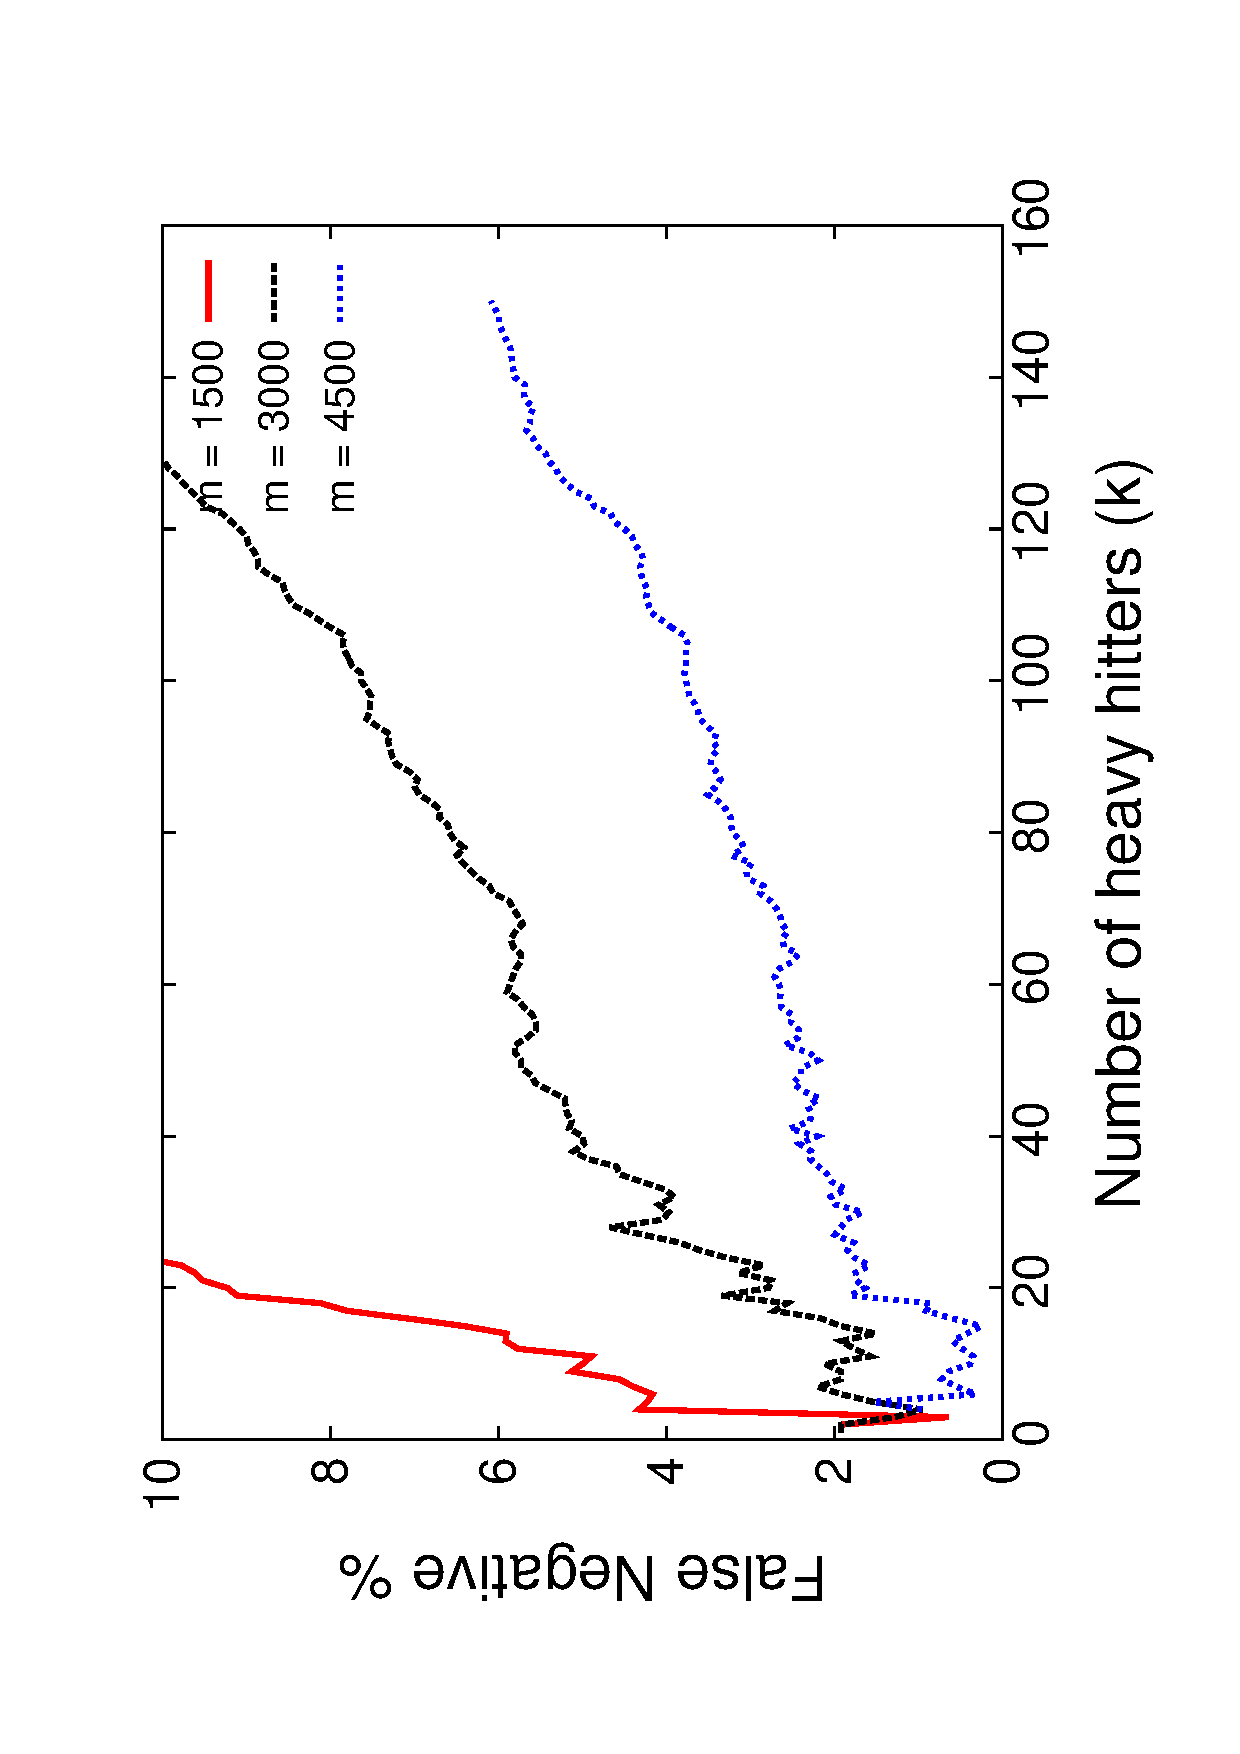
\includegraphics[width=.49\columnwidth]{FalseNegvsKSingle.pdf} &
	\includegraphics[width=.49\columnwidth]{FalseNegvsKTheo.pdf}
    \\
    \mbox{(a) ISP backbone} & \mbox{(b) Data center} \\
  \end{array}
  \]
\caption{False negatives against different numbers of reported heavy flows
  $k$. The heavier a flow is, the less likely that it is missed.}
\label{fig:falseNegvsK}
\end{figure}

% \begin{figure}[ht]
% 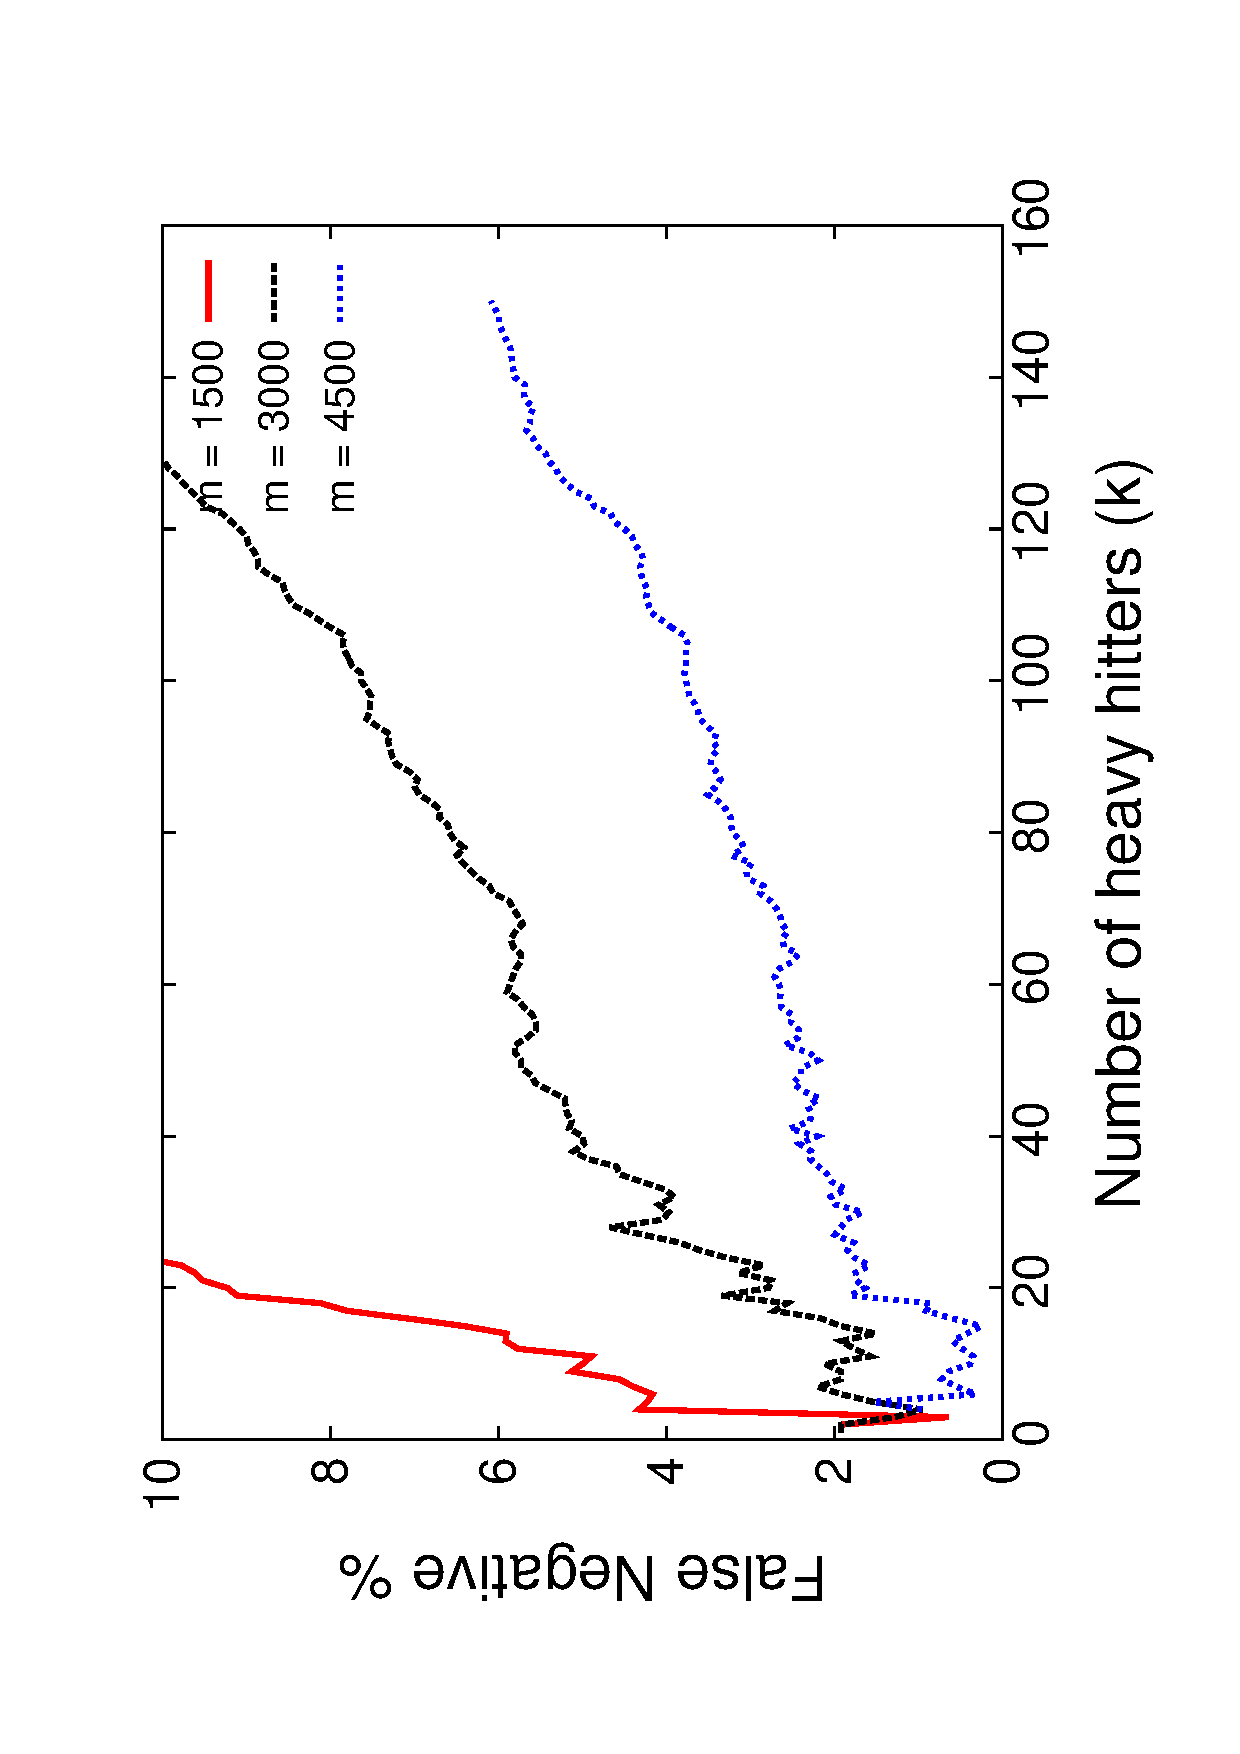
\includegraphics[width=.49\columnwidth]{FalseNegvsKSingle.pdf}
% \includegraphics[width=.49\columnwidth]{FalseNegvsKTheo.pdf}
% \caption{False negatives against different numbers of reported heavy flows
%   $k$. The heavier a flow is, the less likely it is missed.}
% \label{fig:falseNegvsK}
% \end{figure}

\NewPara{False positives.} \Fig{HPPosvsM} shows the false positives of
\TheSystem against varying memory sizes, exhibiting the natural trend of
decreasing error with increasing memory. In particular, we find that with the
ISP trace, false positive rates are very low, partly owing to the large number
of small flows. On all curves, the false positive rate is smaller than 0.1\%,
dropping to lower than 0.01\% at a table size of 80KB. In the data center trace,
we find that the false positive rate hovers under 3\% over a range of
memory sizes and heavy hitters $k$.
%\ngs{Perhaps add counter estimation errors.}

%% \iffalse
%% \begin{figure}[ht]
%% 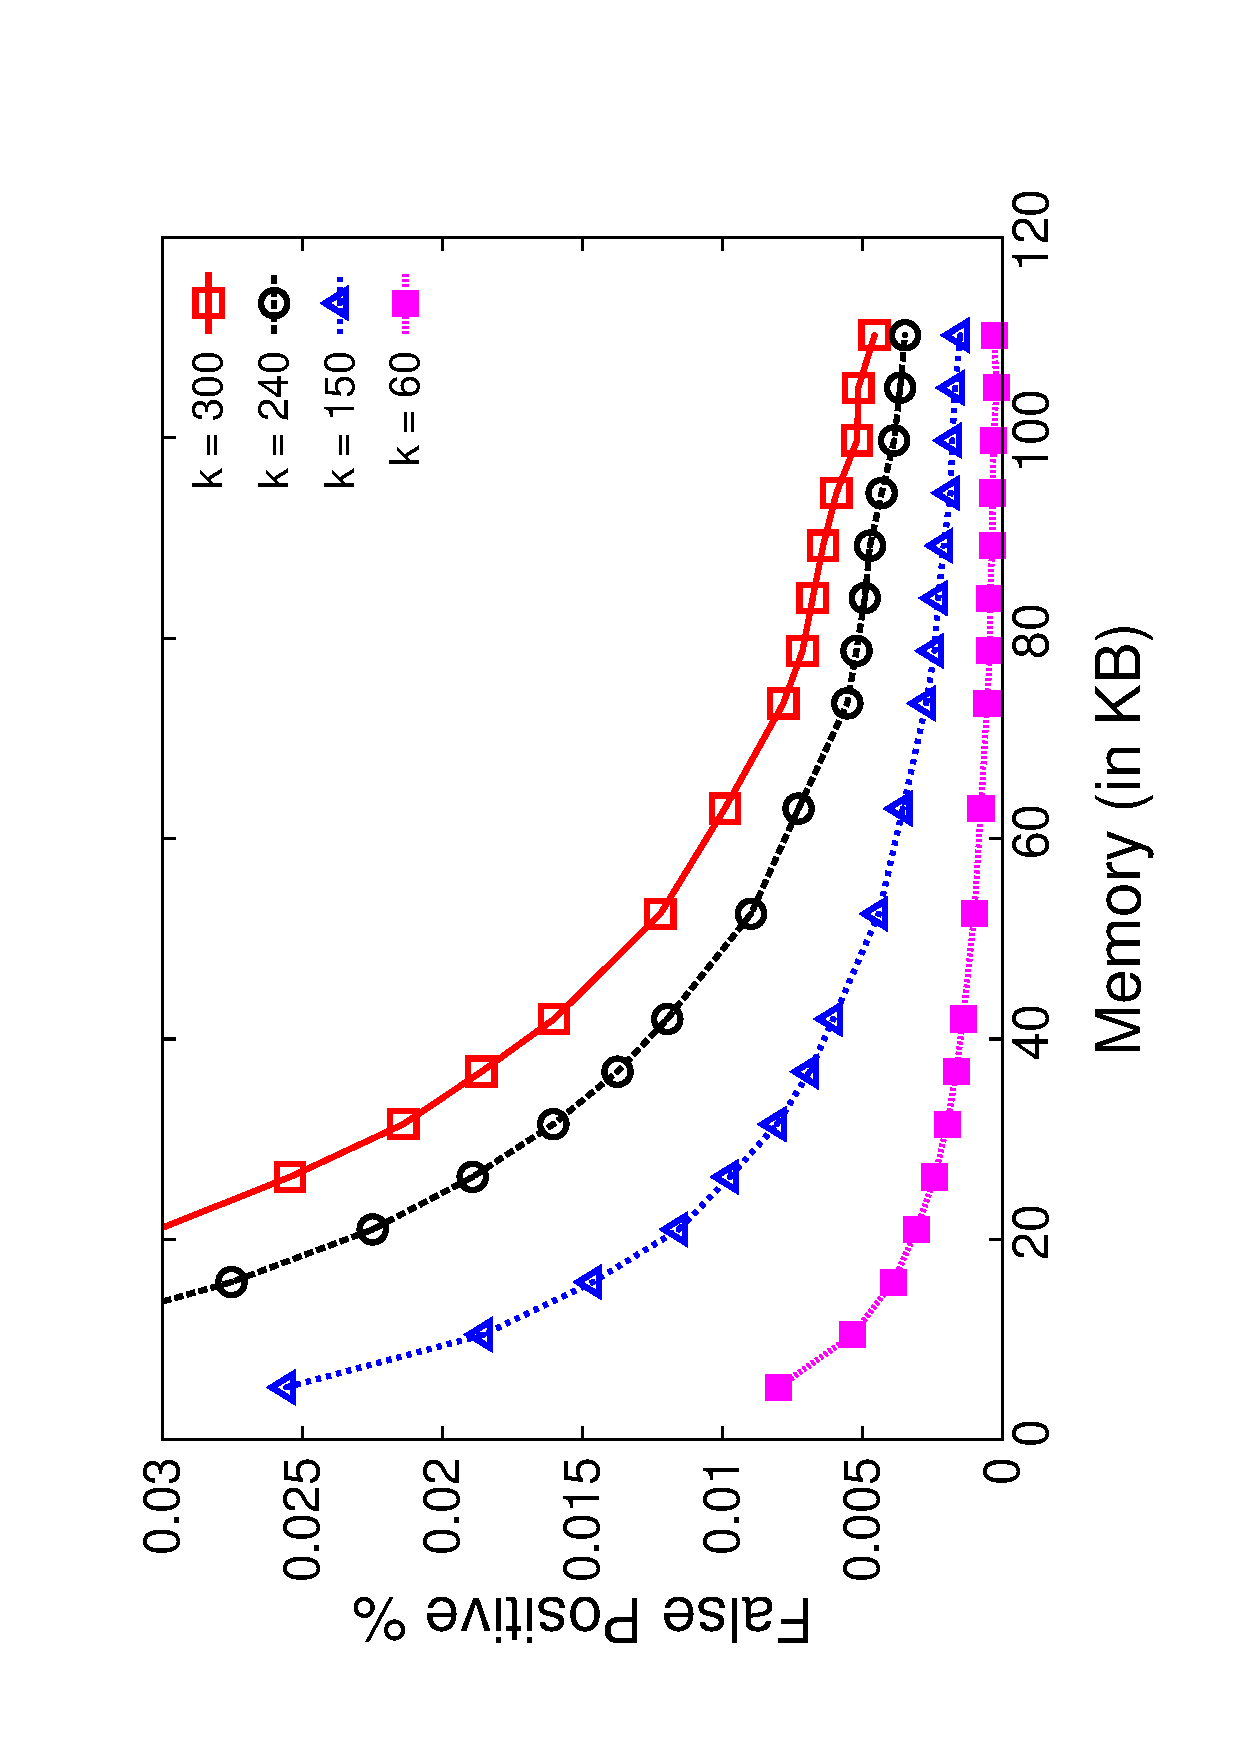
\includegraphics[width=\columnwidth]{FalsePosvsMsSingle.pdf}
%% \caption{\TheSystem has false positive rates of 0.01\%-0.1\% across a range of
%%   table sizes and reported heavy hitters in the ISP trace, and under 1-2\% in
%%   the data center trace.}
%% \label{fig:HPPosvsM}
%% \end{figure}
%% \fi

\begin{figure}
  \centering
  \[
  \begin{array}{ccc}
	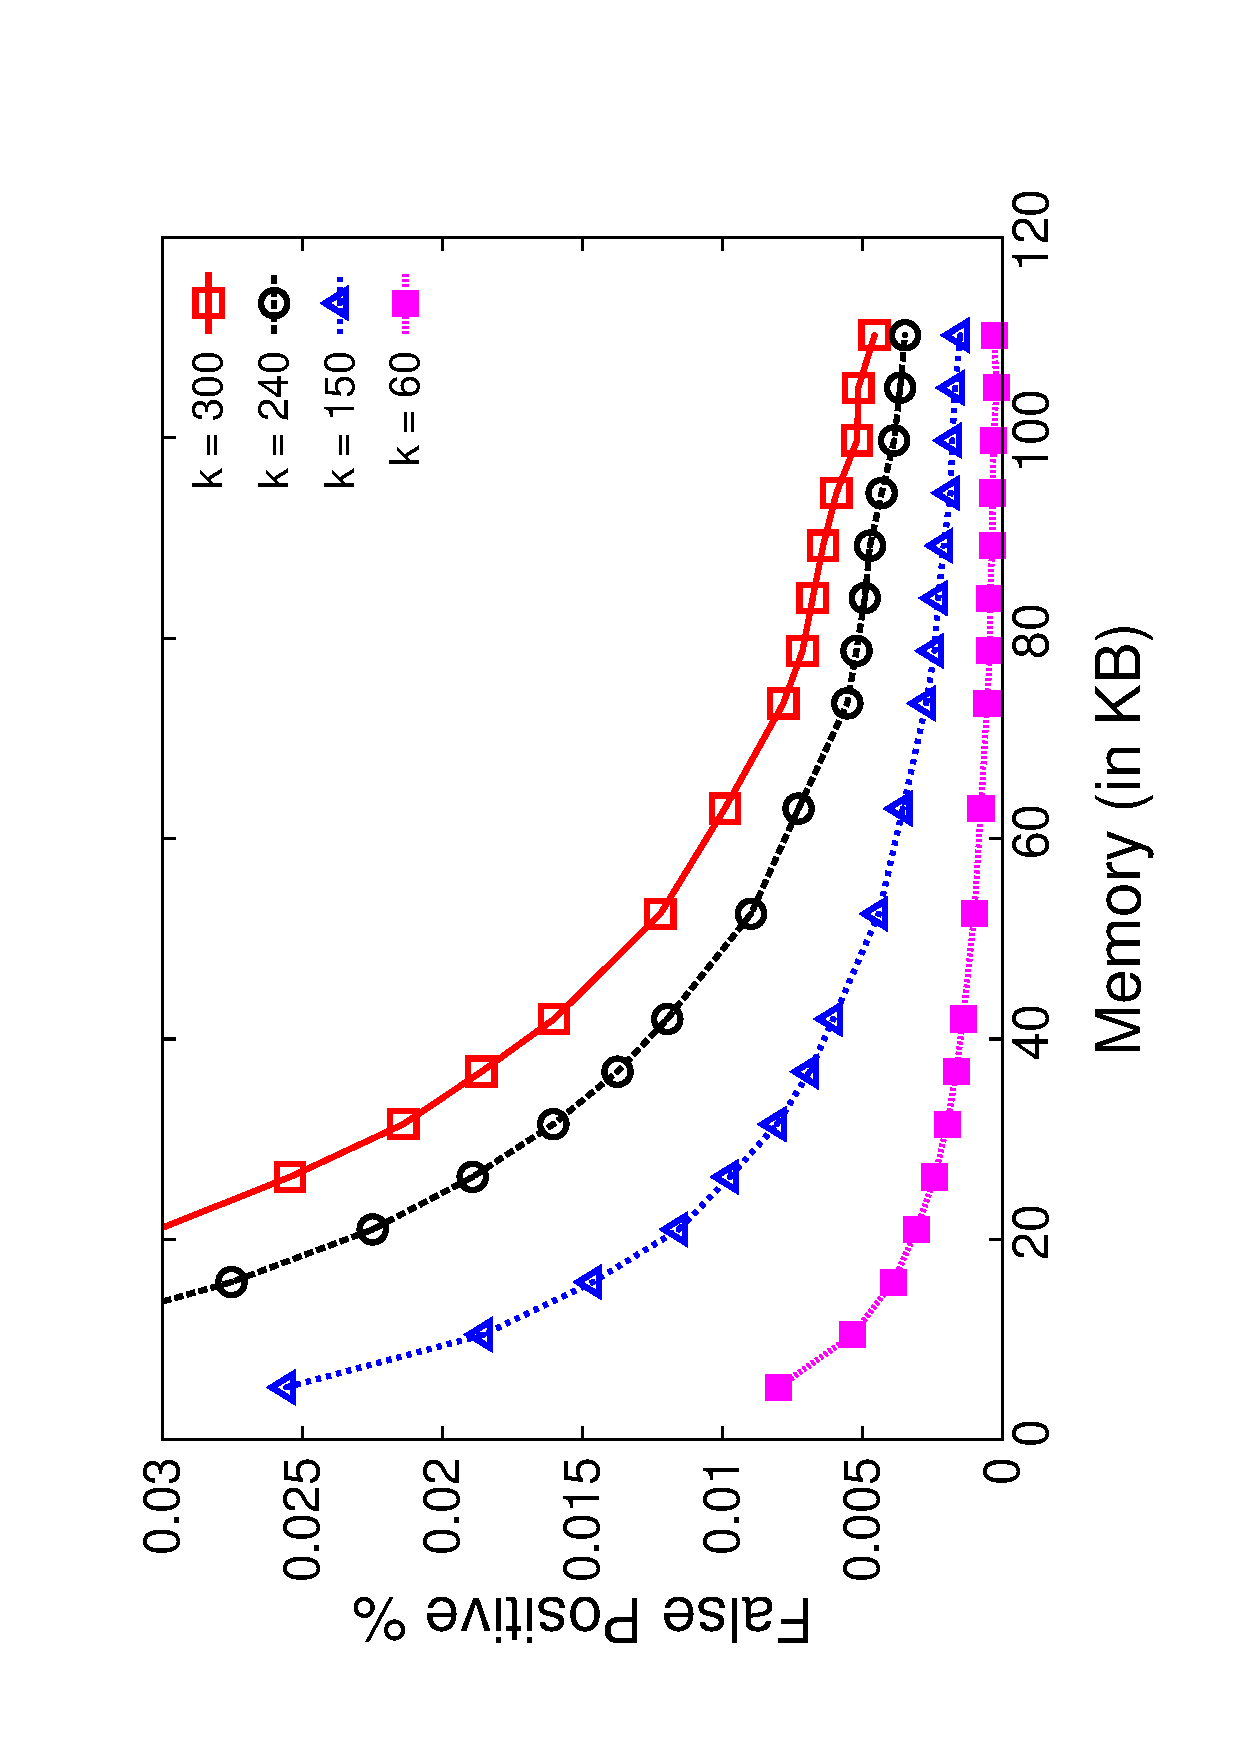
\includegraphics[width=.49\columnwidth]{FalsePosvsMsSingle.pdf} &
	\includegraphics[width=.49\columnwidth]{FalsePosvsMsTheo.pdf}
    \\
     \mbox{(a) ISP backbone} & \mbox{(b) Data center} \\
  \end{array}
  \]
\caption{\TheSystem has false positive rates of 0.01\%-0.1\% across a range of
  table sizes and reported heavy hitters in the ISP trace, and under 3\% in
  the data center trace.}
\label{fig:HPPosvsM}
\end{figure}

%Choose parameters for good performance of our scheme. Given a K (for top K) or threshold (for threshold HH), how do you determine
%- number of table stages? 
%- assymetry - wanna explore this at all?
%- memory size?

%(2) Memory/other overheads - get away with not keeping entire key if the goal
%isn't to report to the controller, but instead to act on hh directly in the
%dataplane

In summary, \TheSystem performs well both with the ISP backbone and data center
traces, recognizing heavy-hitter flows in a timely manner, \ie within 20 seconds
and 1 second respectively, directly in the data plane.

\subsection{\TheSystem\ \vs Existing Solutions}\label{subsec:comparisonRelated}

\NewPara{Comparison baselines.} We compare \TheSystem against two
schemes---representative of sampling and sketching---which are able to estimate
counts in the switch directly (\Sec{sec:related}). We use the same total memory
as earlier, and measure the top $k = 150$ flows. We use the ISP backbone trace
henceforth (unless mentioned otherwise),
and compare \TheSystem with the following baseline schemes.

\noindent (1) Sample and Hold: We simulate sample and hold~\cite{estan2002new}
with a flow table that is implemented as a {\em list}.  As described in
\Sec{sec:related}, we liberally allow incoming packets to look up flow entries
anywhere in the list, and add new entries up to the total memory size. The
sampling probability is set according to the available flow table size,
following recommendations from \cite{estan2002new}.

\noindent (2) Count-min sketch augmented with a `heavy flow' cache: We simulate
the count-min sketch~\cite{cormode2005improved}, but use a flow cache to keep
flow keys and exact counts starting from the packet where a flow is {\em
  estimated to be heavy} from the sketch.\footnote{A simpler
  alternative---mirroring packets with high size estimates from the count-min
  sketch---requires collecting $\approx$ 40\% of the packets in the data center
  trace played at the link rate.}
%
We liberally allow the count-min
sketch to use the offline-estimated exact count of the $k$th heaviest
flow in the trace, as a threshold to identify heavy flows. The flow cache is
implemented as a hash table that retains only the pre-existing flow key on a
hash collision. We allocate half the available memory each to the sketch and the
flow cache.\footnote{We follow guidance from \cite[page
    288]{estan2002new} to split the memory.}

\begin{figure}[h]
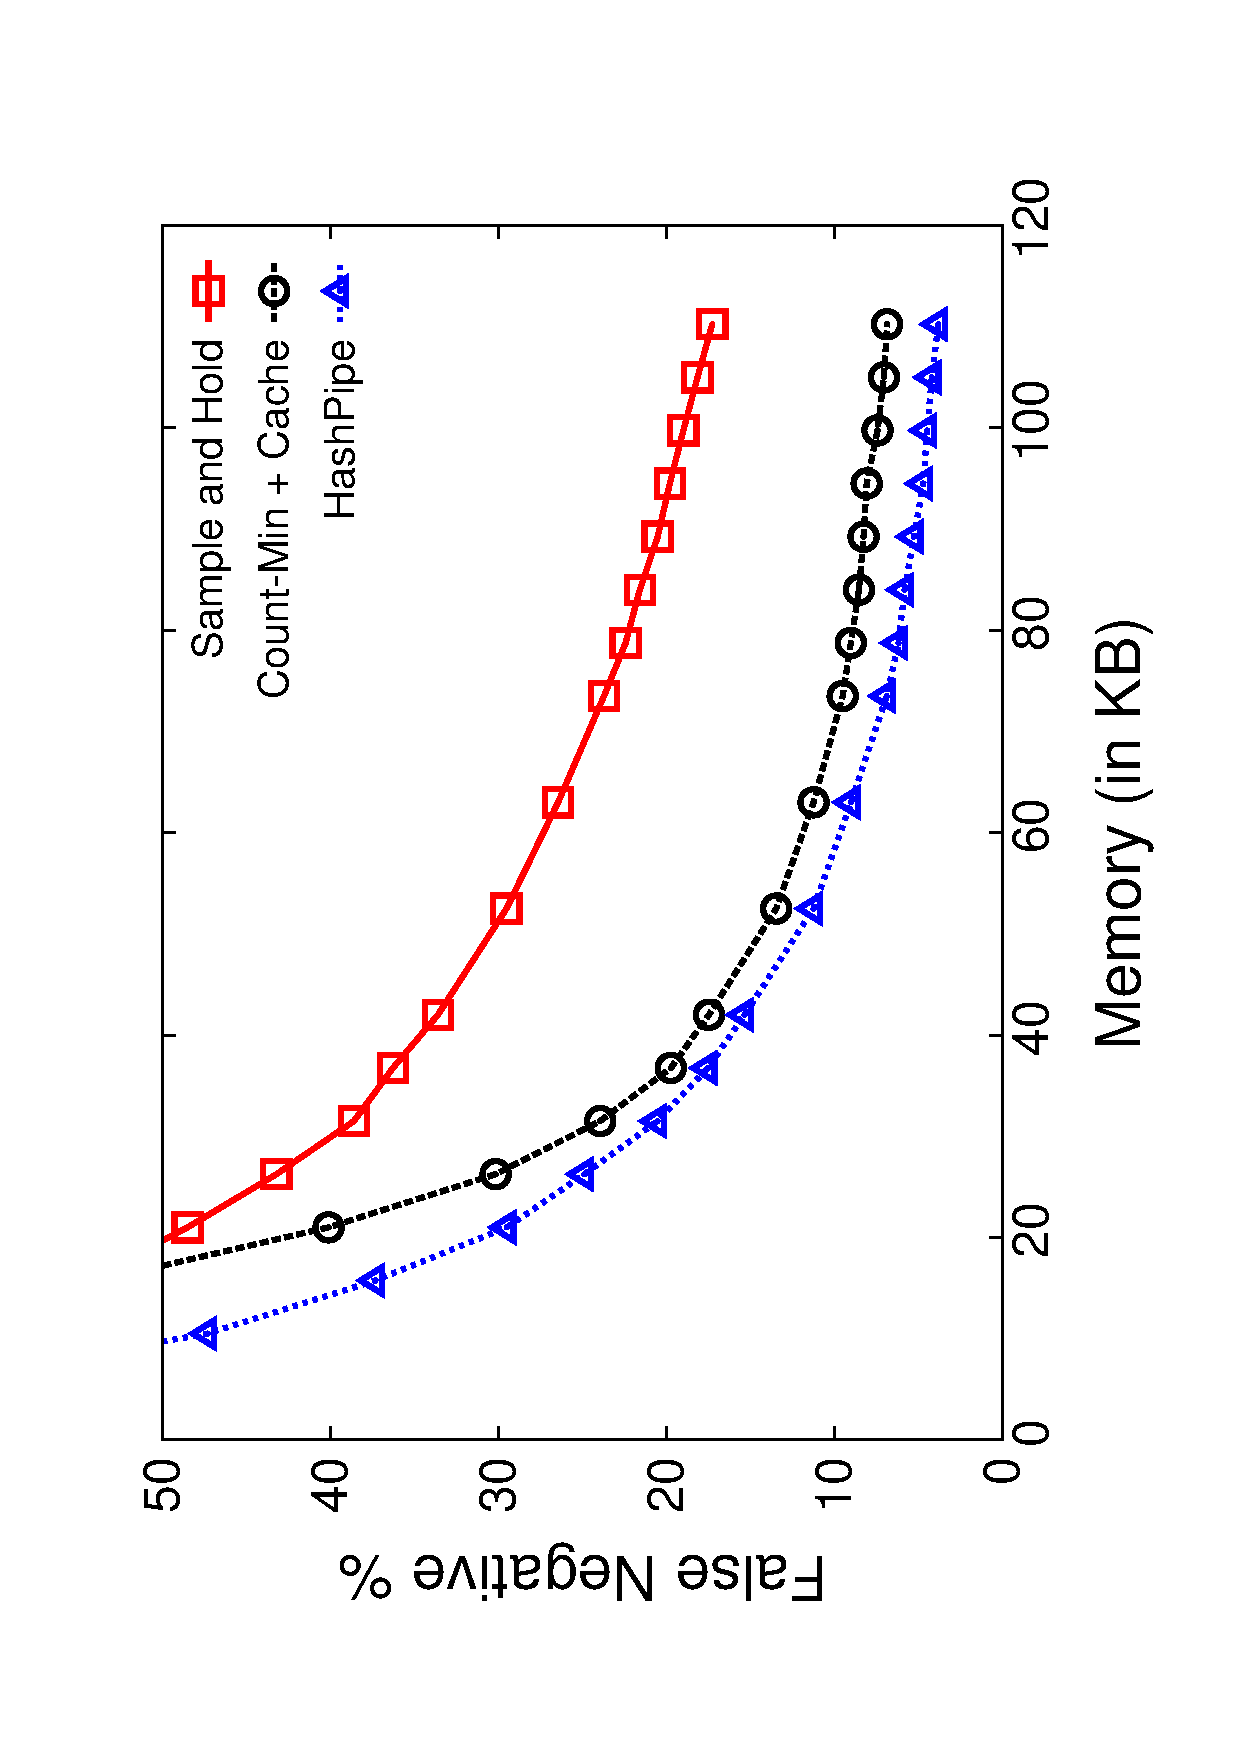
\includegraphics[max height=11cm,max width=8cm]{CompFalseNeg.pdf}
\caption{False negatives of \TheSystem and other
  baselines. \TheSystem outperforms sample and hold and count-min sketch over
  the entire memory range.}
\label{fig:FalseNegvsMSchemes}
\end{figure}

%% In order to evaluate our scheme against our two main competitors, we ran
%% \TheSystem, Count-Min Sketch with a cache and Sample and Hold on the same traces
%% with the same amount of memory (ranging from $5KB$ to $80KB$) and compared the
%% average rate of false negatives that each of the schemes produced across all the
%% traces in detecting the top $150$ flows. In the case of \TheSystem, the memory
%% provisioned is directly translated into a certain number of entries (flowid,
%% packet count pairs) in the hash table assuming that the flow-id is the 5-tuple
%% for an Ipv4 packet. For Sample and Hold, this translates into a similar number
%% of entries based on the same principle, but this is the maximum number of
%% entries that the flow memory can hold \cite{estan2002new}. For the count-min
%% sketch combined with cache, we allocate half of the memory to the sketch itself
%% and the other half to track the heavy-hitter flows in the cache, as suggested in
%% the analysis of the Multi-stage filter \cite{estan2002new}.

\NewPara{False negatives.} \Fig{FalseNegvsMSchemes} shows false negatives
against varying memory sizes, for the three schemes compared. We see that
\TheSystem outperforms sample and hold as well as the augmented count-min sketch
over the entire memory range. (All schemes have smaller errors as the memory
increases.) Notably, at 100KB memory, \TheSystem has 15\% smaller false negative
rate than sample and hold. The count-min sketch tracks the error rate of
\TheSystem more closely from above, staying within a 3-4\% error
difference. Next, we understand where the errors occur in the baseline schemes.

\NewPara{Where are the errors in the other baselines?} \Fig{relative-error}
shows the count estimation error (\%) averaged across flows whose true
  counts are higher than the $x$-value, when running all the schemes with 26KB
  memory.

Sample and hold can make two kinds of estimation errors. It can miss the first
set of packets from a heavy flow because of not sampling the flow early enough,
or (less likely) miss the flow entirely due to not sampling or the flow table
becoming full. \Fig{relative-error} shows that sample and hold makes
the former kind of error even for flows with very high true counts. For
example, there are relative errors of about 10\% even for flows of size more
than 80,000 packets. As \Fig{FalseNegvsMSchemes} shows, the errors becomes less
prominent as the memory size increases, since the sampling rate increases too.

The count-min sketch makes errors because of its inability to discriminate
between heavy and light flows during hash collisions in the sketch. This means
that a {\em light} flow colliding with heavy flows may occupy a flow cache
entry, preventing a heavier flow later on from entering the flow cache. For
instance in \Fig{relative-error}, even flows as large as 50,000 packets can have
estimation errors close to 20\%. However, as \Fig{FalseNegvsMSchemes} shows, the
effect of hash collisions becomes less significant as memory size increases.

On the other hand, \TheSystem's average error on flows larger than 20,000
packets---which is 0.2\% of the total packets in the interval---is negligible
(\Fig{relative-error}). \TheSystem has 100\% accuracy in estimating the count of
flows larger than 30,000 packets.

%% Fig \ref{fig:FalseNegvsMSchemes} suggests that all three schemes uniformly do
%% better at higher amounts of memory. \TheSystem outperforms both Sample and Hold
%% and the Count-min sketch based approach by over $10\%$ at smaller amounts of
%% memory, in terms of missing fewer of the heavy hitting flows. The reason for
%% this is that Sample and Hold only samples one among every so many flows,
%% depending on the sampling rate, which is decided once the flow memory size is
%% decided. Hence, it may lose some of the heavy-hitting flows altogether or may
%% sample a heavy-hitter so late in the measurement interval that its count is
%% underestimated significantly. A more detailed analysis of this effect is
%% illustrated in Figure \ref{fig:relative-error}. 

%% Count-min sketch, on the other hand, does not discriminate between packets
%% belonging to a heavy flow vs. those belonging to a small flow, in maintaining
%% information in the sketch itself. As a consequence, in the count-min sketch
%% and cache scheme, if the smaller flows collide with a few heavy hitters, the
%% heavy hitters' counters themselves are overestimated (Figure
%% \ref{fig:relative-error}) along with the smaller flows occupying the space in
%% the cache that could have gone to true heavy hitters. This effect becomes
%% less prominent as the memory is increased, as Figure
%% \ref{fig:FalseNegvsMSchemes} shows . However, this scheme does rely on
%% setting the threshold for flagging a heavy hitter accurately in the count-min
%% sketch. A lower threshold would result in a lot of flows being added to the
%% cache at the expense of true heavy hitters. A higher threshold would prevent
%% legitimate heavy hitters from even entering the cache. Given that this
%% threshold involves the knowledge of the $k_{th}$ flow's size, this is a
%% somewhat circuitous approach to identifying the $k$ heaviest
%% flows.\vls{unsure if everything is needed}

%
%- sample and hold (currently top K)
%- count min + cache (currently threshold)
%- univmon? opensketch?
%- reversible sketch?
%- XXX: need to figure out exhaustive set of comparison schemes.

\begin{figure}[h]
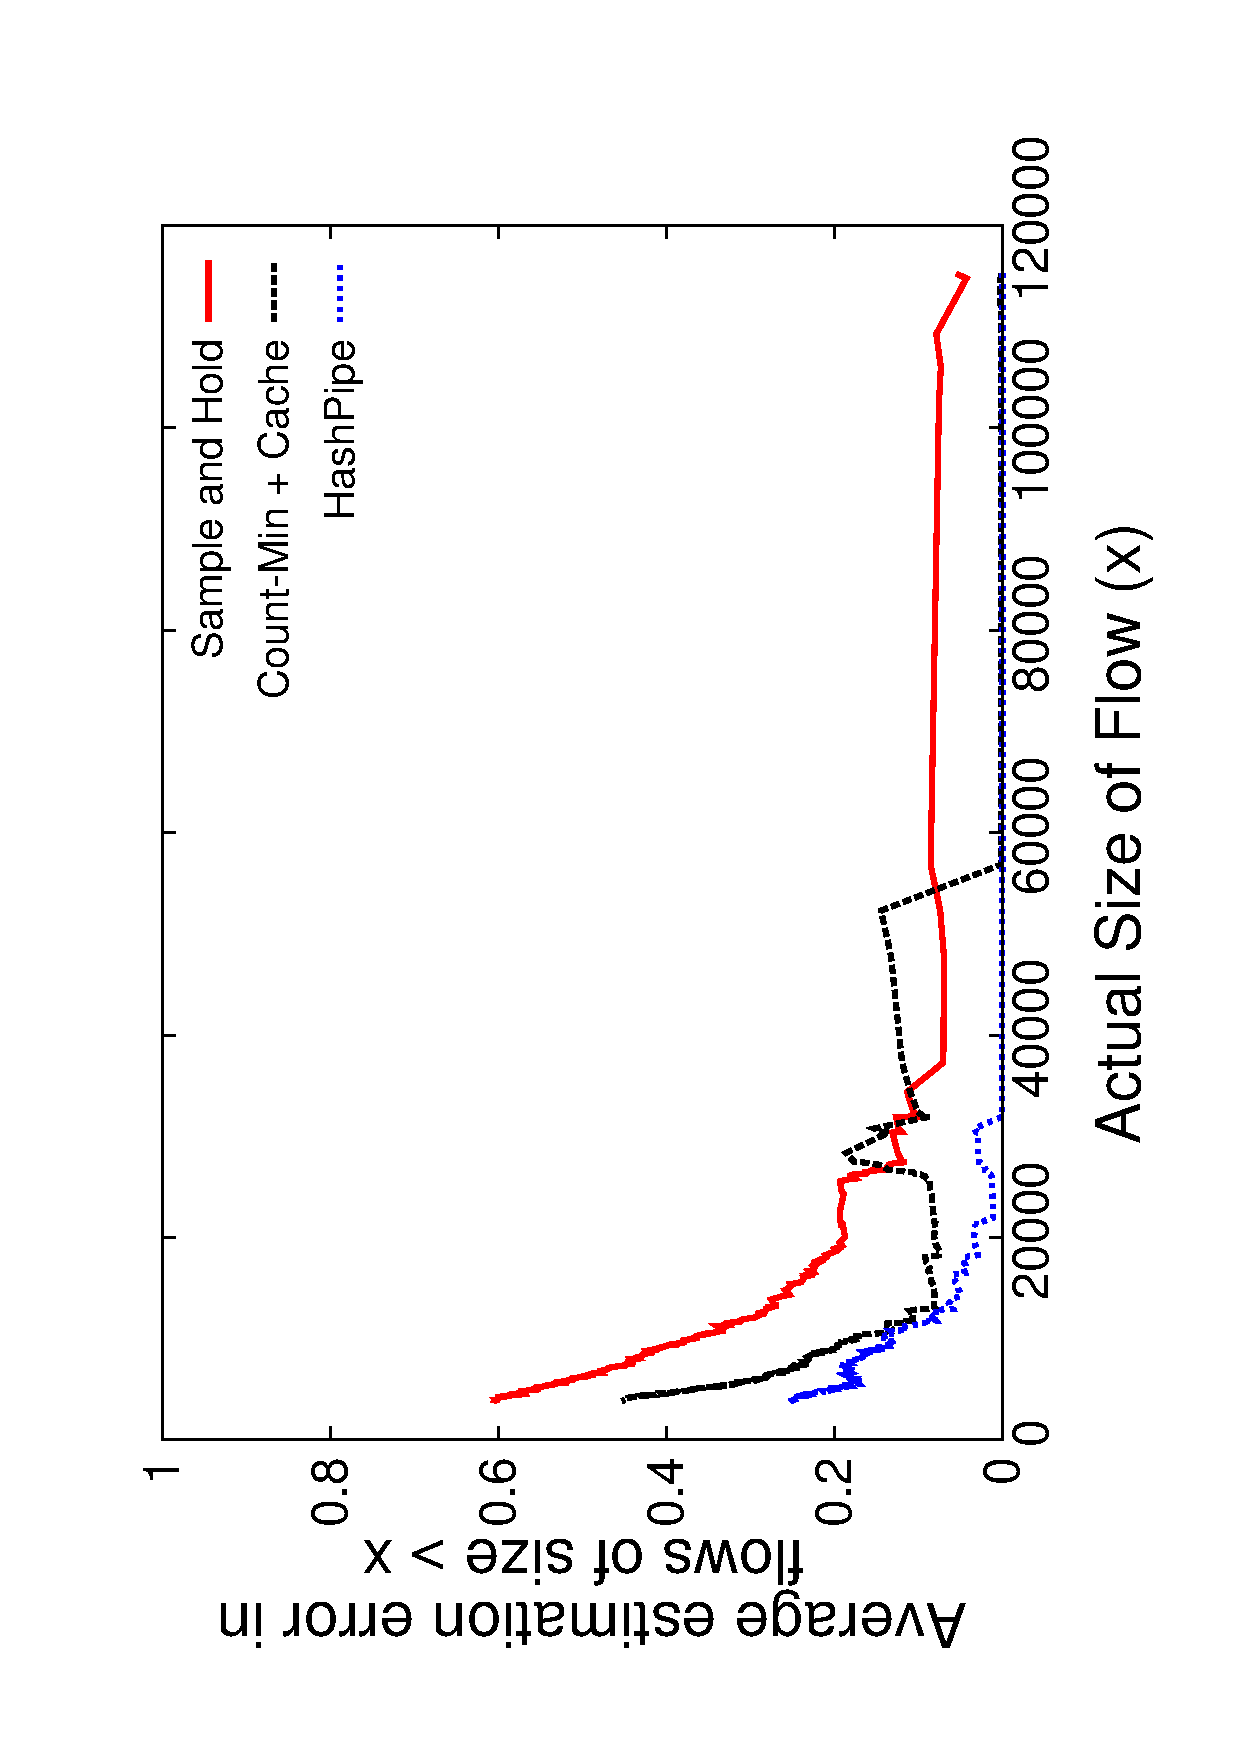
\includegraphics[max height=11cm,max width=8cm]{RelativeError.pdf}
\caption{Comparison of average estimation error (\%) of flows whose true counts
  are higher than the $x$-value in the graph. Sample and hold underestimates
  heavy flows due to sampling, and count-min sketch misses heavy flows due to
  lighter flows colliding in the flow cache. \TheSystem has no estimation errors for
  flows larger than 30,000 packets.}
  %% Comparison of average relative error in the reported sizes of flows whose
  %% actual size is larger than a given actual flow size, when detecting $150$
  %% Heavy Hitters from $0.5M$ flows on average with $26KB$ ofmemory}
\label{fig:relative-error}
\end{figure}

%% Figure \ref{fig:relative-error} analyzes the average relative error in the
%% reporting of all flows larger than a certain size $x$ across all the
%% schemes. Here, the relative error for a given flow of actual size $s_i$ and
%% reported size $r_i$ computed as $|\frac{s_i - r_i}{s_i}|$. The average
%% relative error at size $s$ is then computed as the average among the relative
%% error of all flows that are as large as and larger than $s$. For example, at
%% $x = 20K$ (which is $0.2\%$ of the total number of packets seen in this
%% interval)the average error in the reported size of all flows larger than
%% $20K$ packets is almost negligible with \TheSystem, around $10\%$ of $20K$
%% \ie $2K$ packets with the Count-Min sketch and a cache, and around $20\%$ or
%% $4K$ packets with Sample and Hold. WHle all schemes report higher flows with
%% better accuracy, \TheSystem achieves the almost $100\% $accuracy for all
%% flows of size larger than $30K$, which is faster than the other two. This
%% accounts for its ability to report the heavy hitters more accurately than
%% either of the other two.

\subsection{\TheSystem\ \vs Idealized Schemes}\label{subsec:comparisonIdeal}

We now compare \TheSystem against the idealized algorithms it is derived from
(\Sec{sec:algorithm}), namely \spacesaving~\cite{metwally2005efficient} and
\Baseline.

There are two reasons why \TheSystem may do badly relative to \spacesaving: (i)
it may evict a key whose count is much higher than the table minimum, hence
missing heavy items from the table, and (ii) it may allow too many duplicate
flow keys in the table (\Sec{sec:feed-forward}), reducing the memory available
for heavy flows, and evict heavy flows whose counts are underestimated due to
the duplicates. We showed that duplicate keys are not very prevalent in
\Sec{subsec:sensitivity}; in what follows, we understand their effects on false
negatives in the reported flows.

\NewPara{How far is the subsampled minimum from the true table minimum?}
\Fig{mindist} shows the complementary CDF of the minimum count that was chosen
by \TheSystem, obtained by sampling the algorithm's choice of minimum at every
100th packet in a 10 million packet trace. We don't show the corresponding CCDF
for the absolute minimum in the table, which only takes on two values---0 and
1---with the minimum being 1 more than 99\% likely.\footnote{Note that this is
  different from the minimum of \spacesaving, whose distribution contains much
  larger values.}
%
We see that the chance that \TheSystem chooses a certain minimum value decreases
rapidly as that value grows, judging from the straight-line plot on log scales
in \Fig{mindist}.
%
For example, the minimum counter has a value higher than 5 less than 5\% of the
time. There are a few larger minimum values (\eg 100), but they are rarer (less
than 0.01\% of the time). This suggests that it is unlikely that \TheSystem
experiences large errors due to the choice of a larger minimum from the table,
when a smaller counter exists.
%% srinivas: we haven't discussed why the absolute minimum distribution is so
%% skewed: possibly because we always insert keys with values 1. It seems less
%% important, though.

\begin{figure}[h]
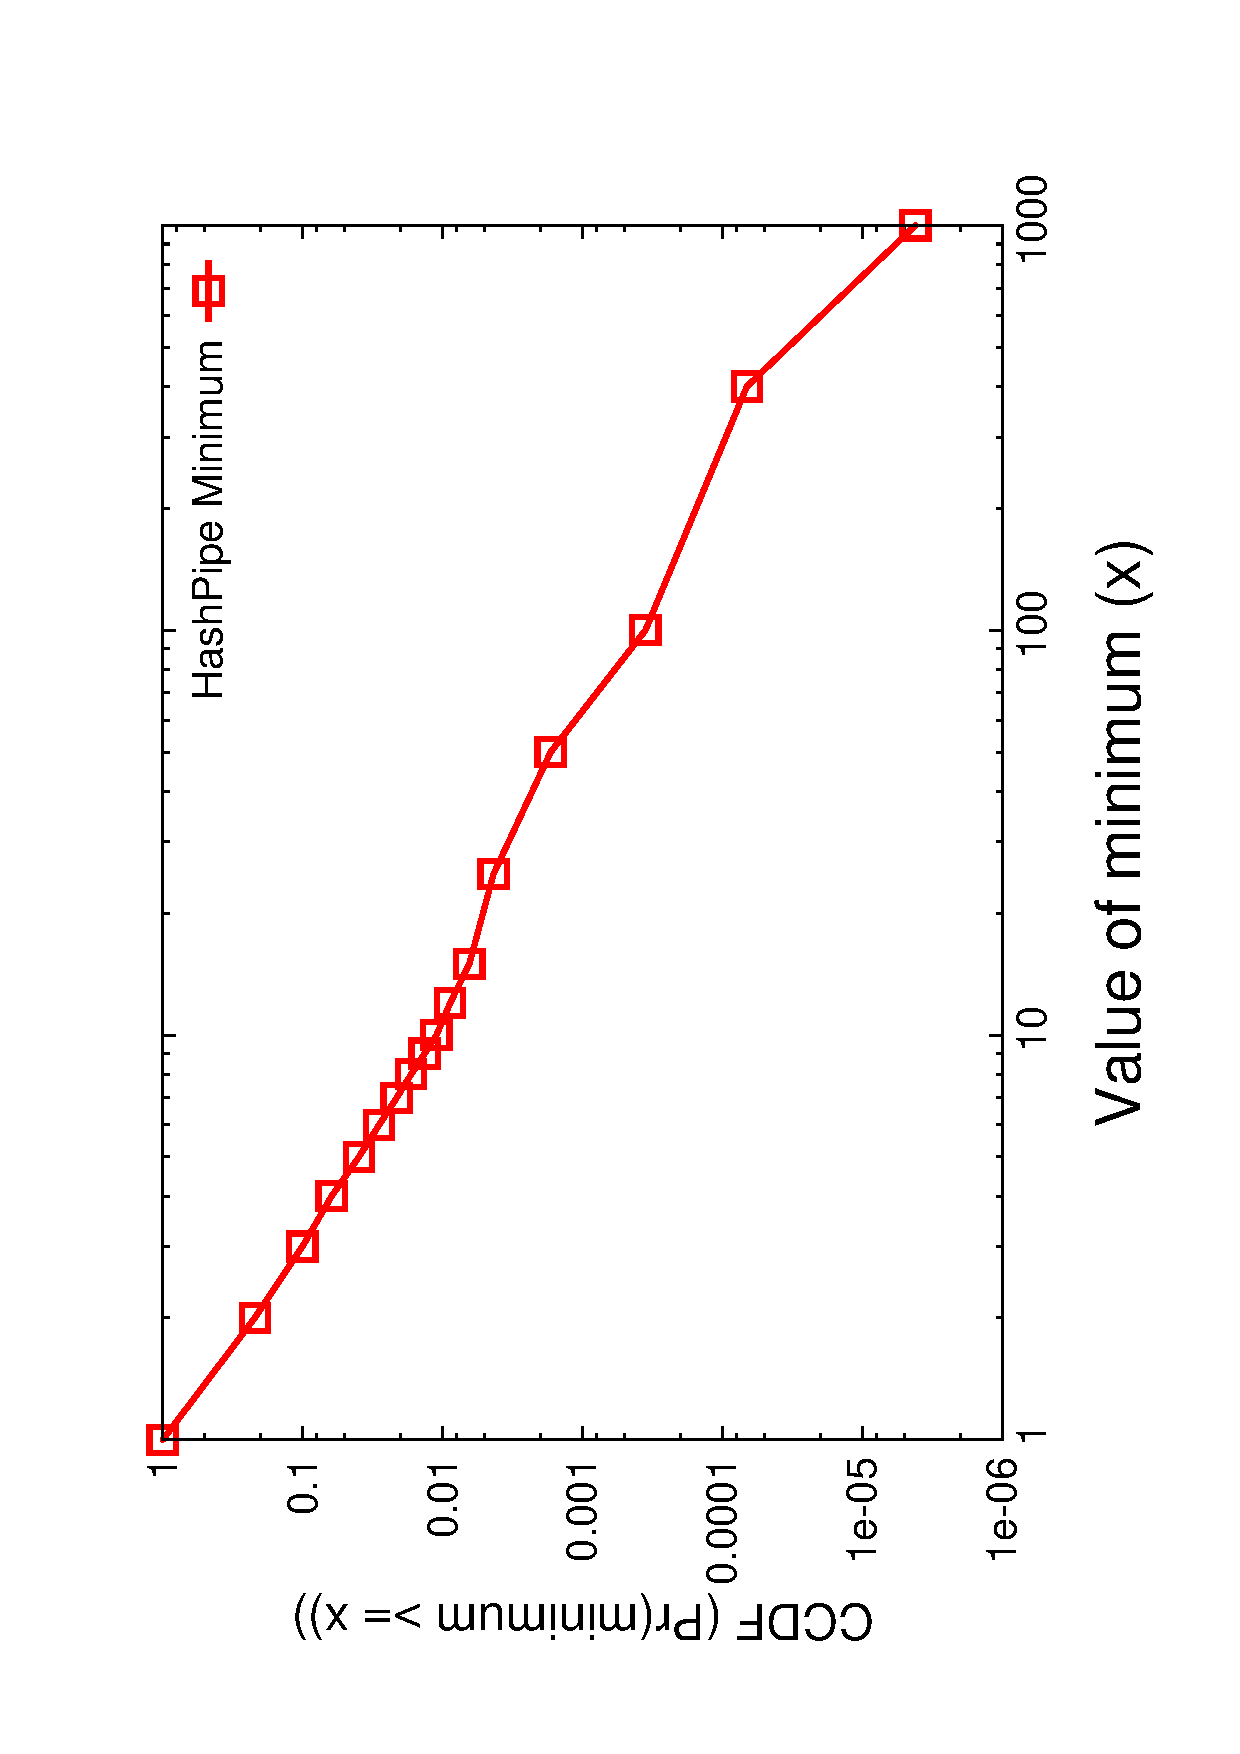
\includegraphics[max height=11cm,max width=8cm]{minDistribution.pdf}
\caption{Complementary CDF of the minimum chosen by \TheSystem on $26KB$ of
  memory, sampled every 100th packet from a trace of 10 million packets.}
\label{fig:mindist}
%plot CM, UnivMon, Reversible
\end{figure}

%% \TheSystem aims to model the Space Saving \cite{metwally2005efficient}
%% algorithm in a hardware-amenable version by sampling a few locations to
%% estimate the minimum instead of computing the global minimum. A natural
%% question to ask is how far are we in our minimum approximation fromt the
%% global minimum. We compared the minimum picked by \TheSystem with the actual
%% minimum in the table at the same-time for the hash table update corresponding
%% to every $100_{th}$ packet in the trace. Figure \ref{fig:mindist} shows the
%% complementary cumulative distribution function for the two minima. The two
%% distributions look reasonably similar indicating that the approximated
%% minimum isn't that far off from the actual minimum and it is very rarely
%% higher than $10$. Further, the true minimum of the table is almost always $1$
%% which is also expected since we insert flows with value $1$ in the first
%% table stage. Our scheme also reports $1$ as the actual minimum majority of
%% the time.

\begin{figure}[h]
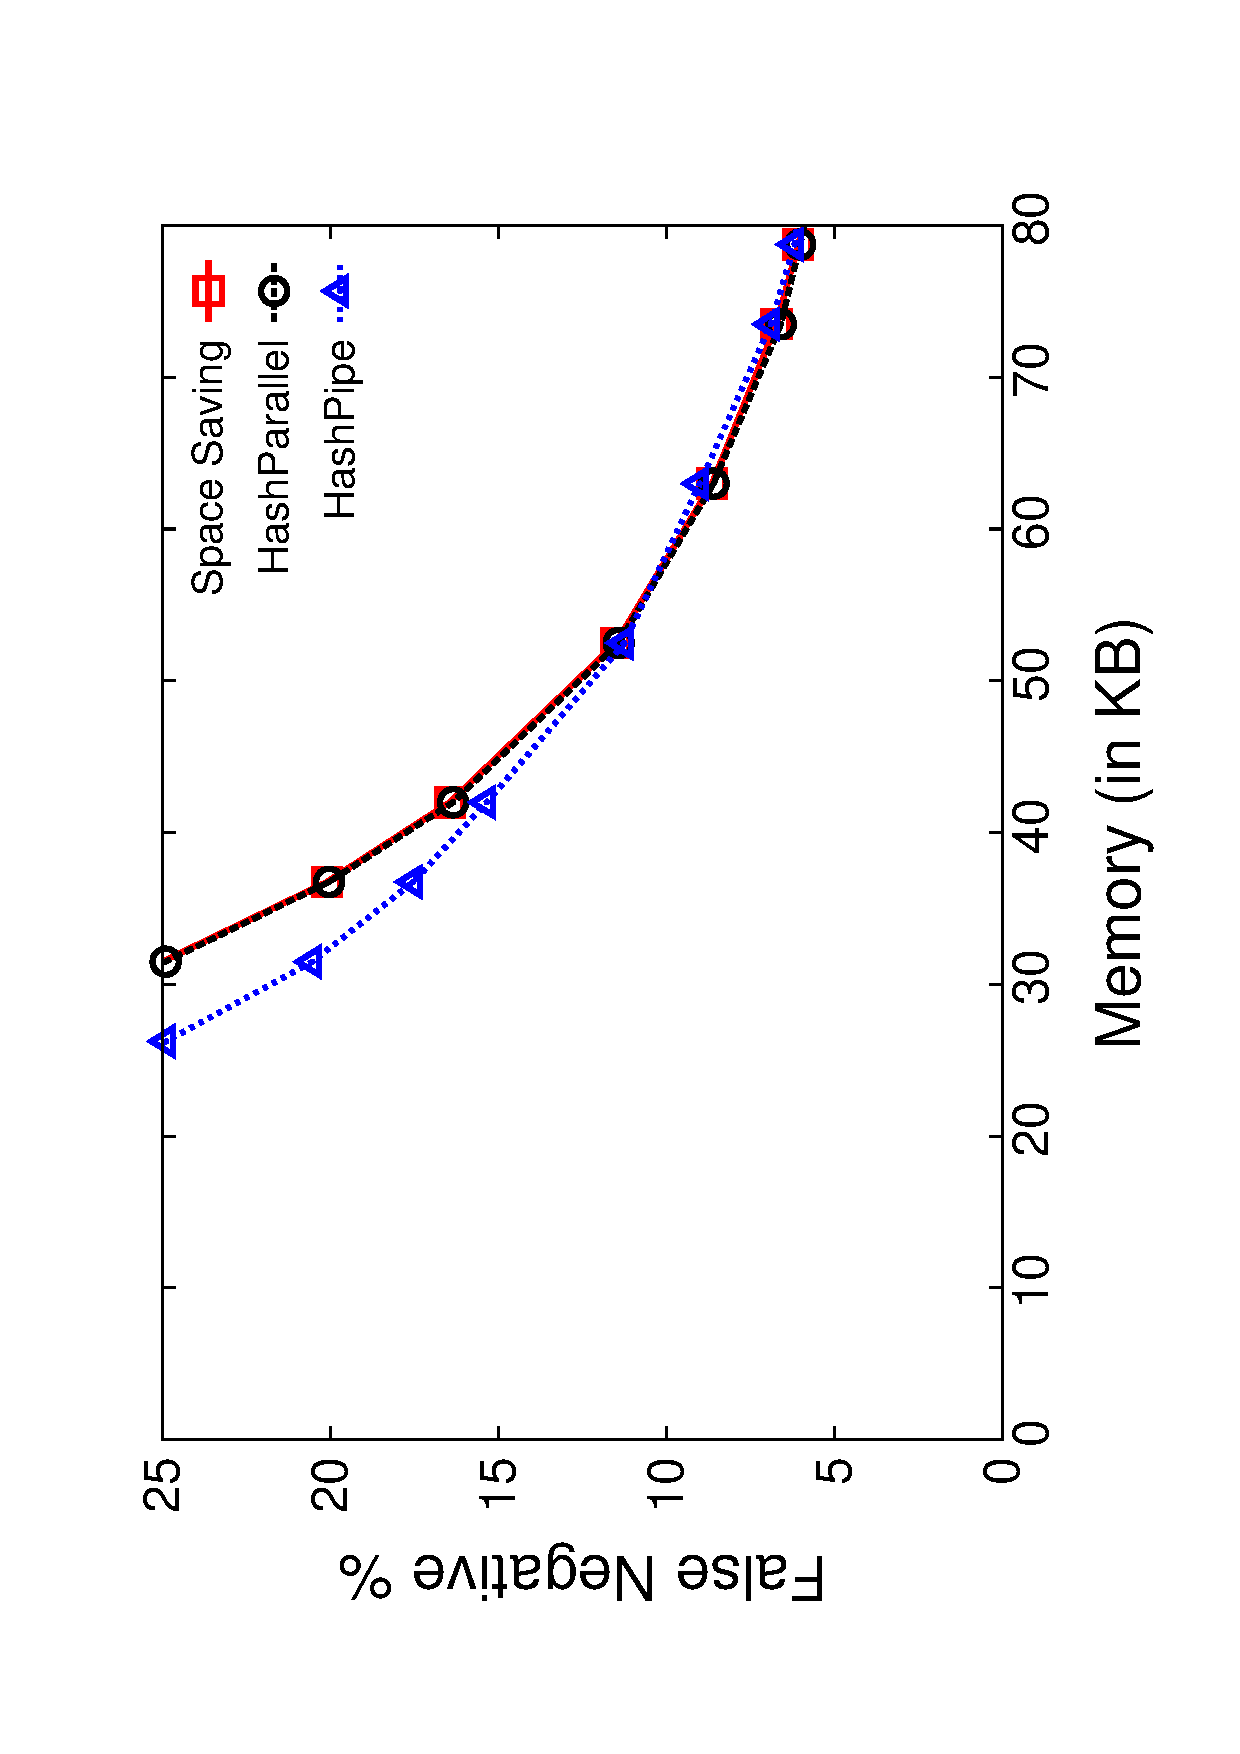
\includegraphics[max height=11cm,max width=8cm]{FriendsFalseNeg.pdf}
\caption{Comparison of false negatives of \TheSystem to idealized schemes when
  detecting $k$=150 heavy hitters. In some memory regimes, \TheSystem may
  even outperform \spacesaving, while \Baseline closely tracks \spacesaving.}
%% \caption{False Negative Rate for memory sizes when detecting $150$ heavy hitters from $0.5M$ flows across $10M$ packets}
\label{fig:FalseNegvsFriendSchemes-k150}
%plot CM, UnivMon, Reversible
\end{figure}


\begin{figure}[h]
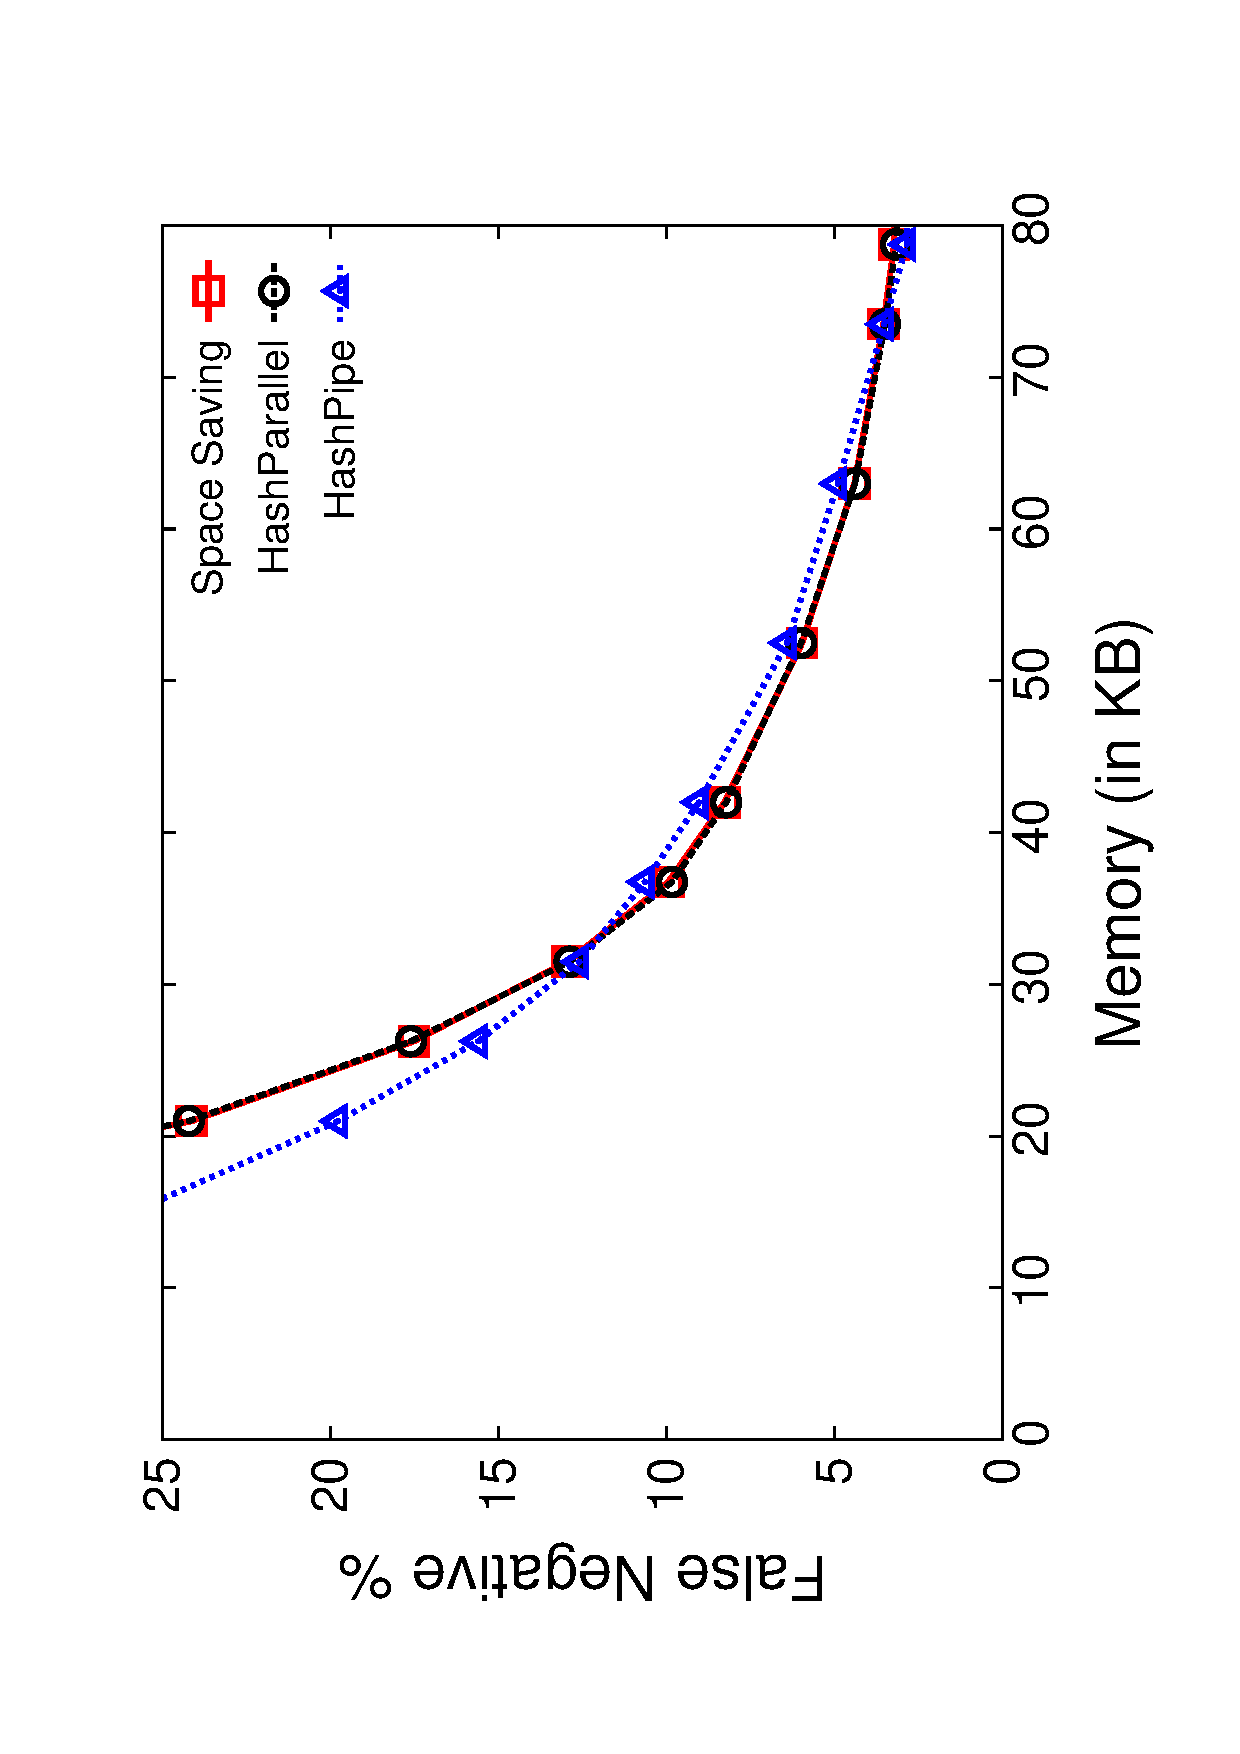
\includegraphics[max height=11cm,max width=8cm]{FriendsFalseNeg60.pdf}
\caption{Comparison of false negatives of \TheSystem to idealized schemes when
  detecting $k$=60 heavy hitters.}
%% \caption{False Negative Rate for memory sizes when detecting $60$ heavy hitters
%%   from $0.5M$ flows across $10M$ packets}
\label{fig:FalseNegvsFriendSchemes-k60}
%plot CM, UnivMon, Reversible
\end{figure}

\NewPara{Comparison against \spacesaving and \Baseline.} We compare the false
negatives of the idealized schemes and \TheSystem against varying memory sizes
in \Fig{FalseNegvsFriendSchemes-k150} and \Fig{FalseNegvsFriendSchemes-k60},
when reporting two different number of heavy hitters, $k$=150 and $k$=60
respectively. Two features stand out from the graph for both $k$ values. First,
wherever the schemes operate with low false negative error (say less than 20\%),
the performance of the three schemes is comparable (\ie within 2-3\% of each
other). Second, there are small values of memory where \TheSystem\ {\em
  outperforms} \spacesaving.

Why is \TheSystem outperforming \spacesaving? \Spacesaving only guarantees that
the $k$th heaviest item is in the table when the $k$th item is larger than the
average table count (\Sec{sec:spacesaving}). In our trace, the 60th item and
150th item contribute to roughly 6000 and 4000 packets out of 10 million
(resp.), which means that they require at least\footnote{10 million / 6000
  $\approx$ 1700; 10 million / 4000 $\approx$ 2500.} 1700 counters and 2500
counters in the table (resp.). These correspond to memory sizes of 30KB and 45KB
(resp.). At those values of memory, we see that \spacesaving starts
outperforming \TheSystem on false negatives.

We also show why \spacesaving fails to capture the heavier flows when it is
allocated a number of counters smaller than the minimum number of counters
mentioned above. Note that \TheSystem attributes every packet to its flow entry
correctly (but may miss some packets entirely), since it always starts a new
flow at counter value 1. However, \spacesaving increments {\em some counter} for
every incoming packet (\Alg{spacesaving}). In contexts where the number of
active flows is much larger than the number of available counters (\eg 400,000
flows with 1200 counters), this can lead to some flows having enormously large
(and grossly overestimated) counters. In contrast, \TheSystem keeps the counter
values small for small flows by evicting the flows (and counts) entirely from
the table.

At memory sizes smaller than the thresholds mentioned above, incrementing a
counter for each packet may result in {\em several small flows} catching up to a
heavy flow, leading to significant false positives, and higher likelihood of
evicting truly heavy flows from the table. We show this effect on \spacesaving
in \Fig{SSkeysperbucket} for $k$=150 and $m$=1200 counters, where 
in fact $m=2500$ counters are required as described earlier.
%
The distribution of the number of keys contributing to a false positive flow
counter in the table is clearly shifted to the right relative to the
corresponding distribution for a true positive.
%
%% A similar and
%% natural characterization of the distributions holds for the estimation errors
%% from the different categories of flow keys, shown in \Fig{SSdevperbucket}.

%% To quantify how we do compared to \spacesaving, we compared the performance of
%% \TheSystem against the intermediate \Baseline as well as \spacesaving in terms
%% of the false negative rate in the reporting of $150$ heavy hitters with
%% different amounts of memory. As reported in Figure
%% \ref{fig:FalseNegvsFriendSchemes}, \Baseline is almost identical to \spacesaving
%% in its performance. This is not surprising since Figure \ref{fig:mindist} shows
%% that sampling the minimum doesn't result in such a different distribution from
%% the actual minimum. However, \TheSystem has significantly lower false negative
%% rates (by almost $15\%$) than either of them at almost all memory sizes. This is
%% attributed to the fact that \TheSystem inserts a new flow with value $1$ in the
%% first table while \spacesaving and \Baseline both replace it with the current
%% minimum value incremented by $1$.

\begin{figure}[h]
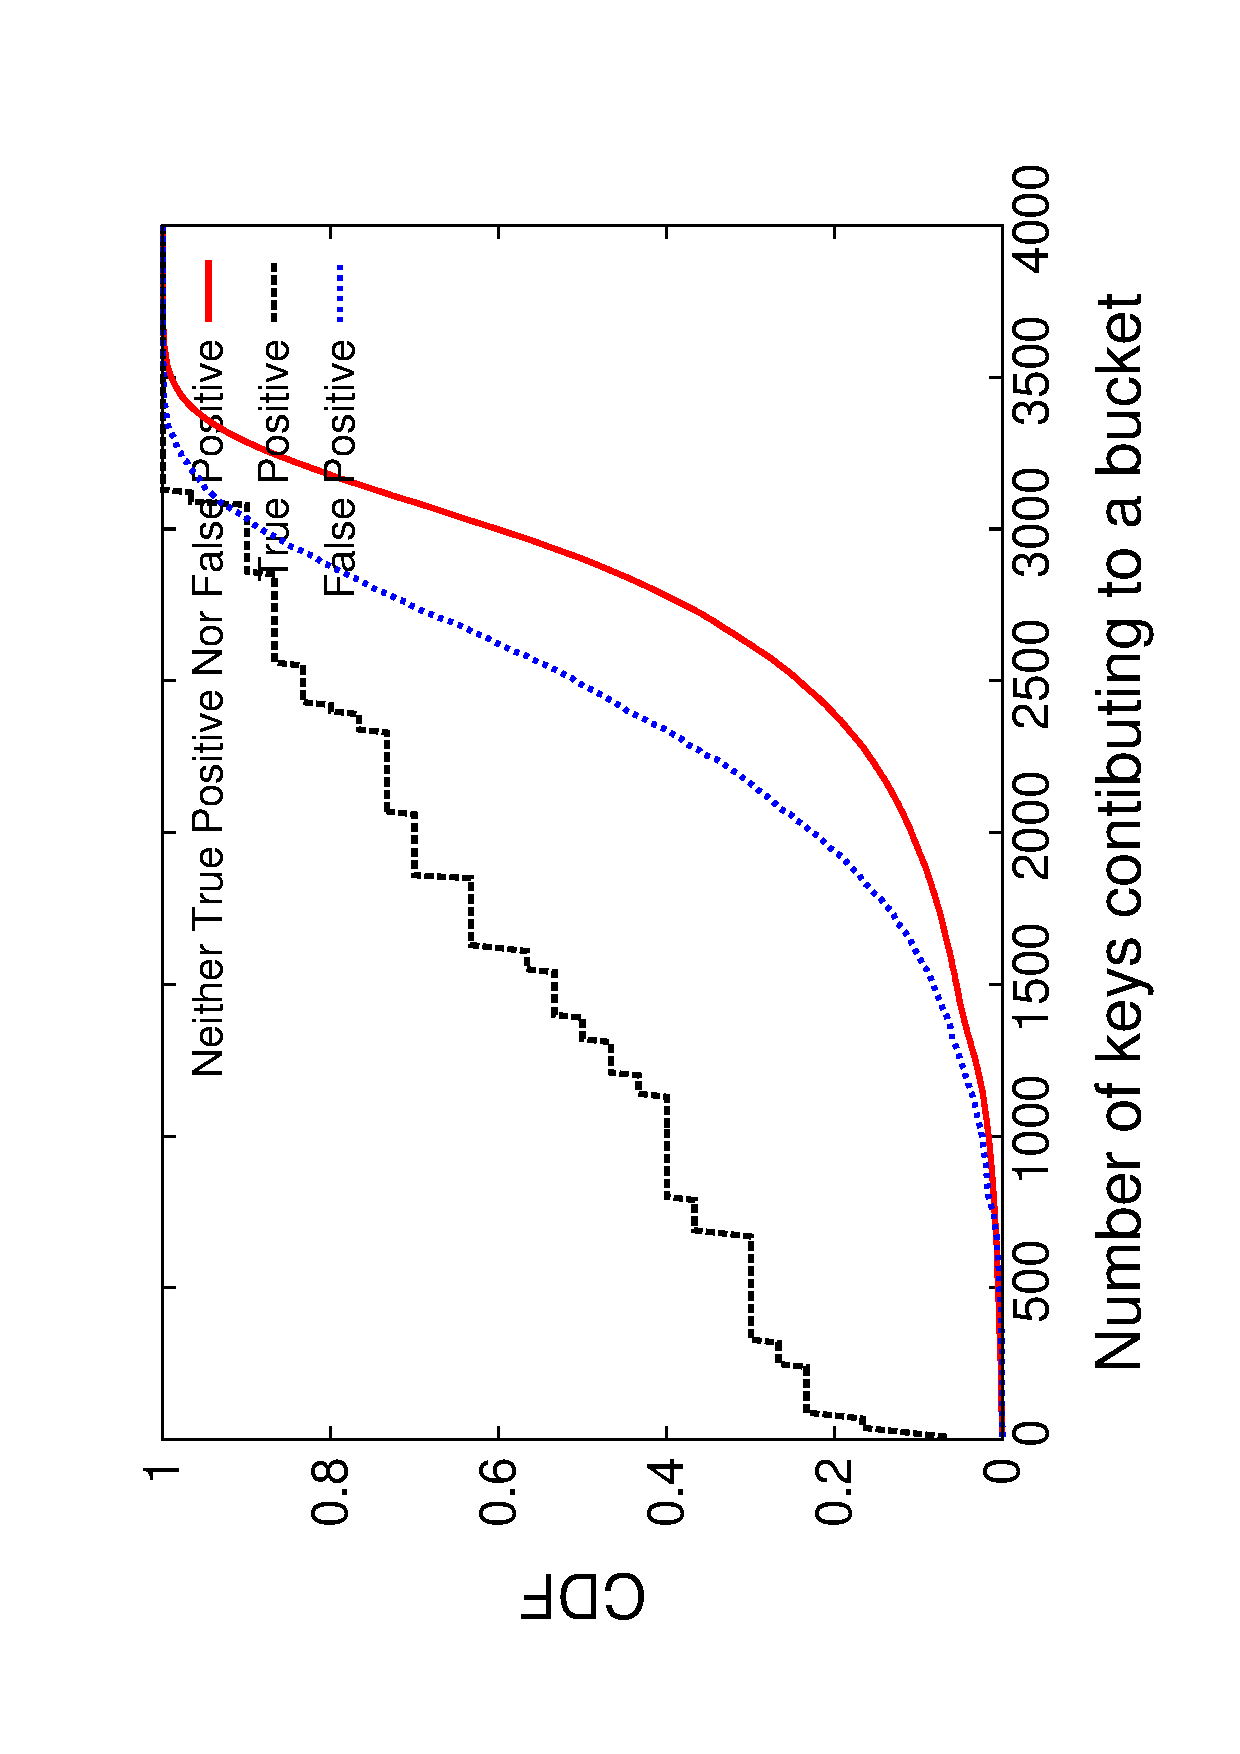
\includegraphics[max height=11cm,max width=8cm]{SSKeysPerBucketDist.pdf}
\caption{CDF of the number of distinct flows contributing to a counter in
  \spacesaving's table, when identifying $k$=150 heavy flows with $m$=1200
  counters. We show three distributions according to the flow's label after the
  experiment.}
%% \caption{Chances of a given bucket having a certain number of keys contributing
%%   to it when running \spacesaving to identify $150$ heavy hitters with $1200$
%%   counters. Legend represents category that the flow found in a bucket at the
%%   end of the interval belongs to.}
\label{fig:SSkeysperbucket}
\end{figure}

%% When the number of flows and packets in a network are high (around two orders
%% of magnitude more than the number of entries in the table), the fact that
%% every packet causes at least one counter to increment by $1$
%% \cite{metwally2005efficient} without any evictions results in a large average
%% counter value.  This large average counter could be even larger than some of
%% the heavy hitter flows resulting in certain mice flows being incorrectly
%% reported while other legitimate hevay hitters are missed. To analyze this, we
%% observed the number of keys that contributed to the count in every bucket at
%% the end of the measurement interval in Space-Saving when run with $1200$
%% counters. In addition, we analyzed what the reported size of the flow in the
%% bucket was and how it compared to the actual size of the flow (relative error
%% of that flow). We then classified the flows based on whether they were True
%% Positives, False Positives or neither in the context of the top $150$ flows.

%% \begin{figure}[h]
%% 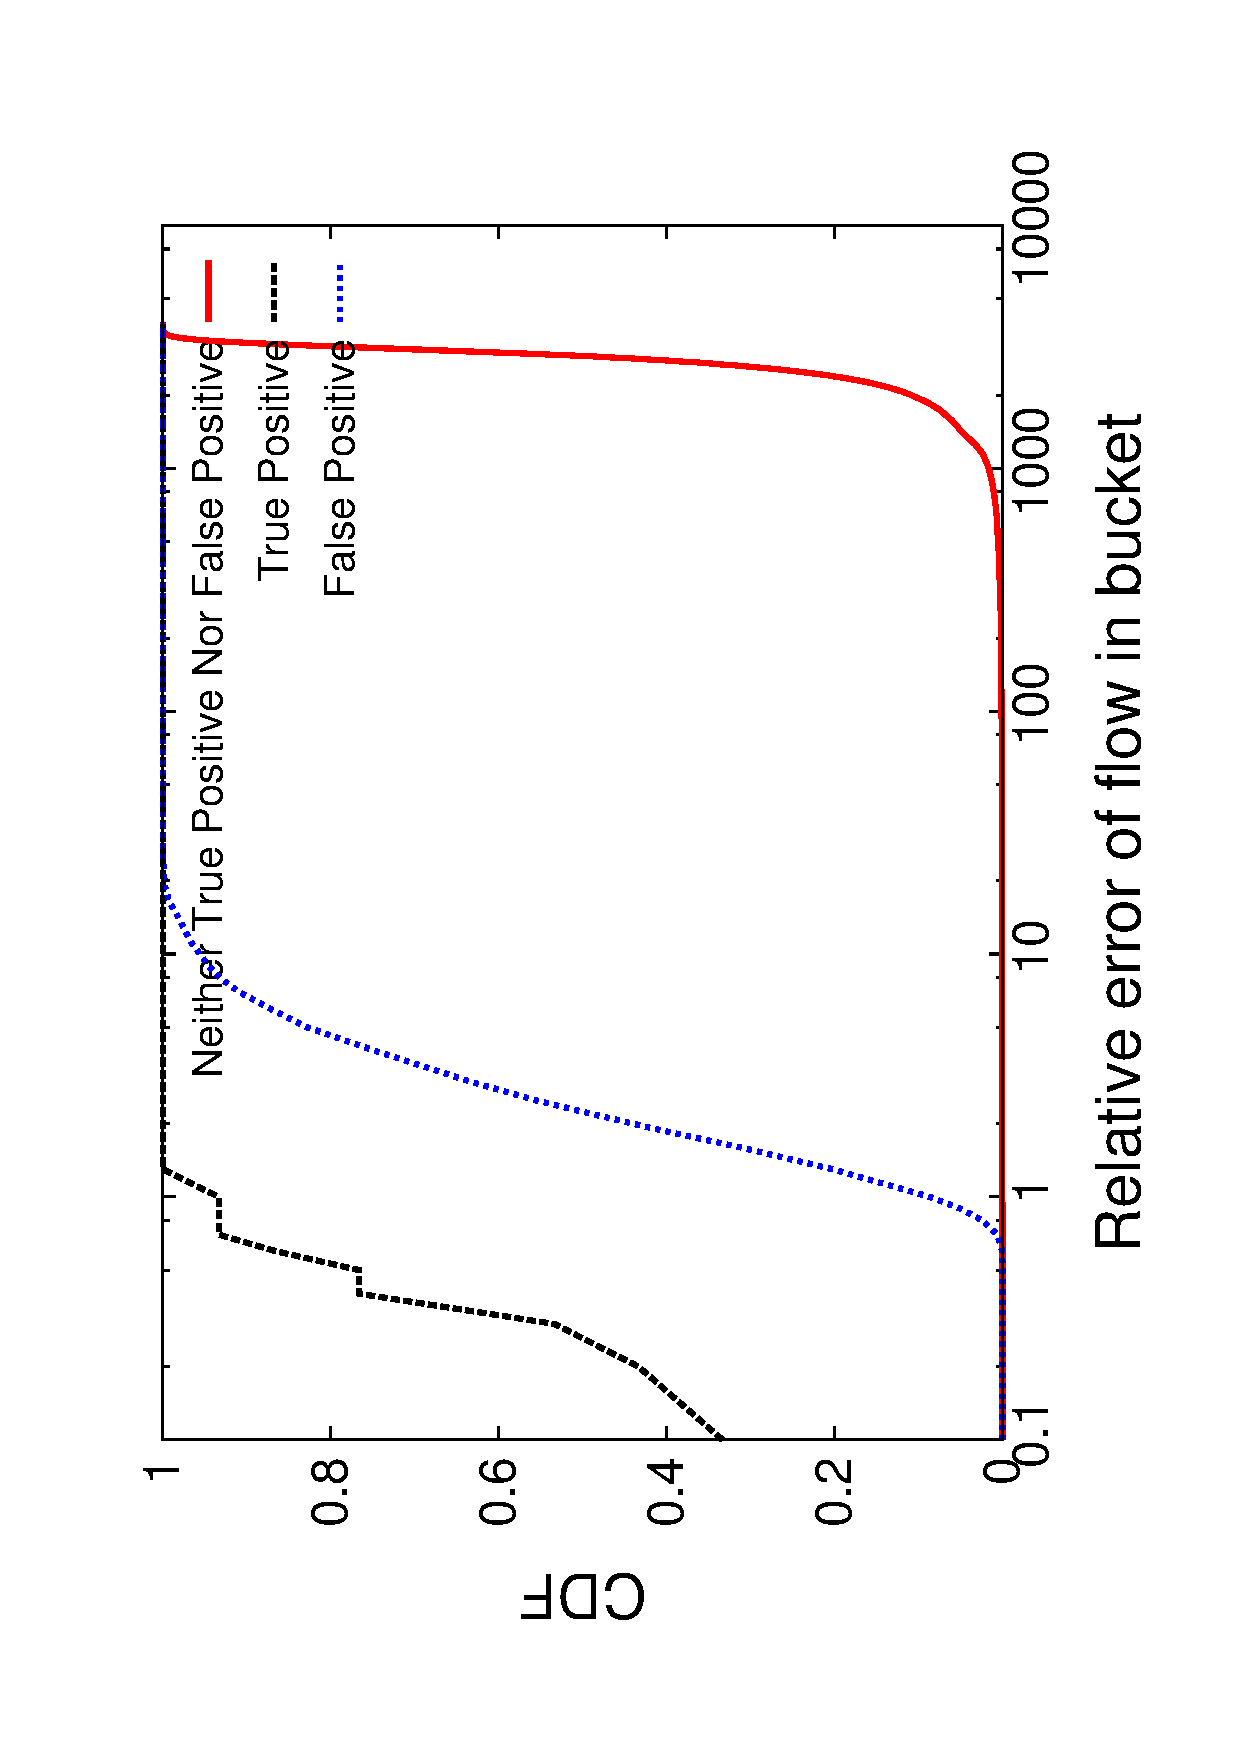
\includegraphics[max height=11cm,max width=8cm]{SSDeviationPerBucketDist.pdf}
%% \caption{CDF of the count estimation error (\%) of different flows in
%%   \spacesaving's table, when identifying $k$=150 heavy flows with $m$=1200
%%   counters. We show three distributions according to the flow's label after the
%%   experiment.}
%% \label{fig:SSdevperbucket}
%% \end{figure}

%% Figure \ref{fig:SSkeysperbucket} shows that the number of keys contributing to a
%% particular bucket is over $2000$ in more than half the buckets. If each of those
%% keys contributed even two packets, that would be over the actual true count of
%% the average $150^{th}$ ranked flow. Thus even a few such buckets would start
%% competing heavily against the true heavy hitters, as illustrated in the false
%% positive line of the plot. Similarly, according to Figure
%% \ref{fig:SSdevperbucket}, the relative error with those flows in the table that
%% are not true positives is so high that it indicates the possibility that if
%% these were medium-sized in the first place, they could, once again, easily
%% replace the true-positives.

\NewPara{Impact of duplicate keys in the table.} Finally, we investigate how
duplicate keys and consequent underestimation of flow counts in the table may
affect the errors of \TheSystem. In \Fig{reportingMoreThanK-falseneg}, we show
the benefits of reporting {\em more than $k$ counters} on false negatives, when
the top $k$=300 flows are requested with a memory size of $m$=2400 counters.
While the false negative rates of \spacesaving and \Baseline improve
significantly with overreporting, the errors for \TheSystem remains flat
throughout the interval, dropping only around 1800 reported flows. We infer that
most heavy flows are retained somewhere in the table for \spacesaving and
\Baseline, while \TheSystem underestimates keys sufficiently often that they are
completely evicted---to the point where overreporting does not lower the false
negative errors.
%
%% \Fig{reportingMoreThanK-falsepos} shows that 
We find that overreporting
flows only increases the false positive errors slightly for all schemes, with
values staying between 0.1-0.5\% throughout.

\begin{figure}[h]
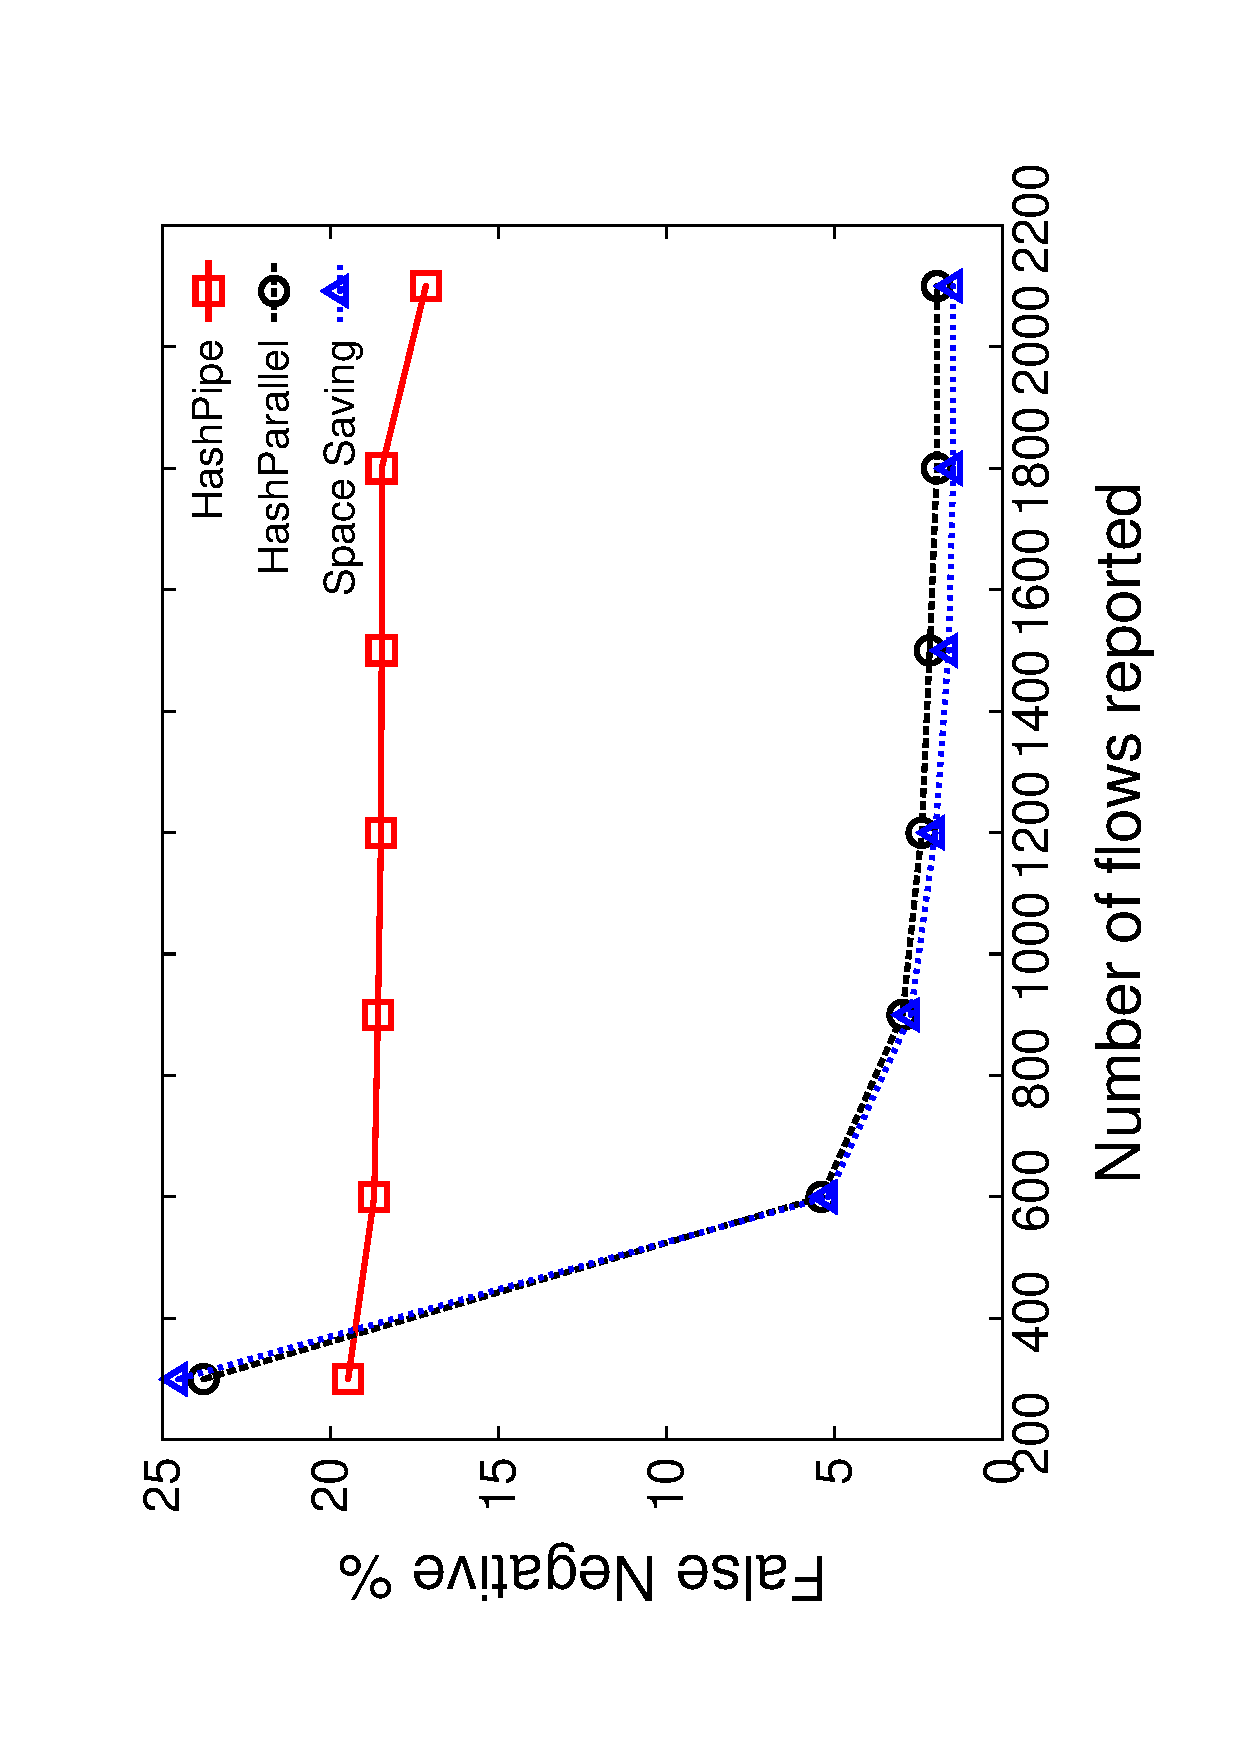
\includegraphics[max height=11cm,max width=8cm]{FriendsFalseNegWithRep.pdf}
\caption{Benefits of overreporting flows on false negative errors
  with $k$=300 heavy flows and $m$=2400 counters. While \spacesaving and
  \Baseline improve significantly by reporting even $2k$ flows,
  \TheSystem does not, because of evictions due to duplicate entries.}
%% \caption{
%%   Comparison of false negatives of HashPipe to \spacesaving and Hash
%%   Parallel when reporting more than $k$ candidate flows. \spacesaving and
%%   HashParallel significantly outperform HashPipe even with $2k$ reported flows}
\label{fig:reportingMoreThanK-falseneg}
\end{figure}

\iffalse
\begin{figure}[h]
%width=.49\columnwidth
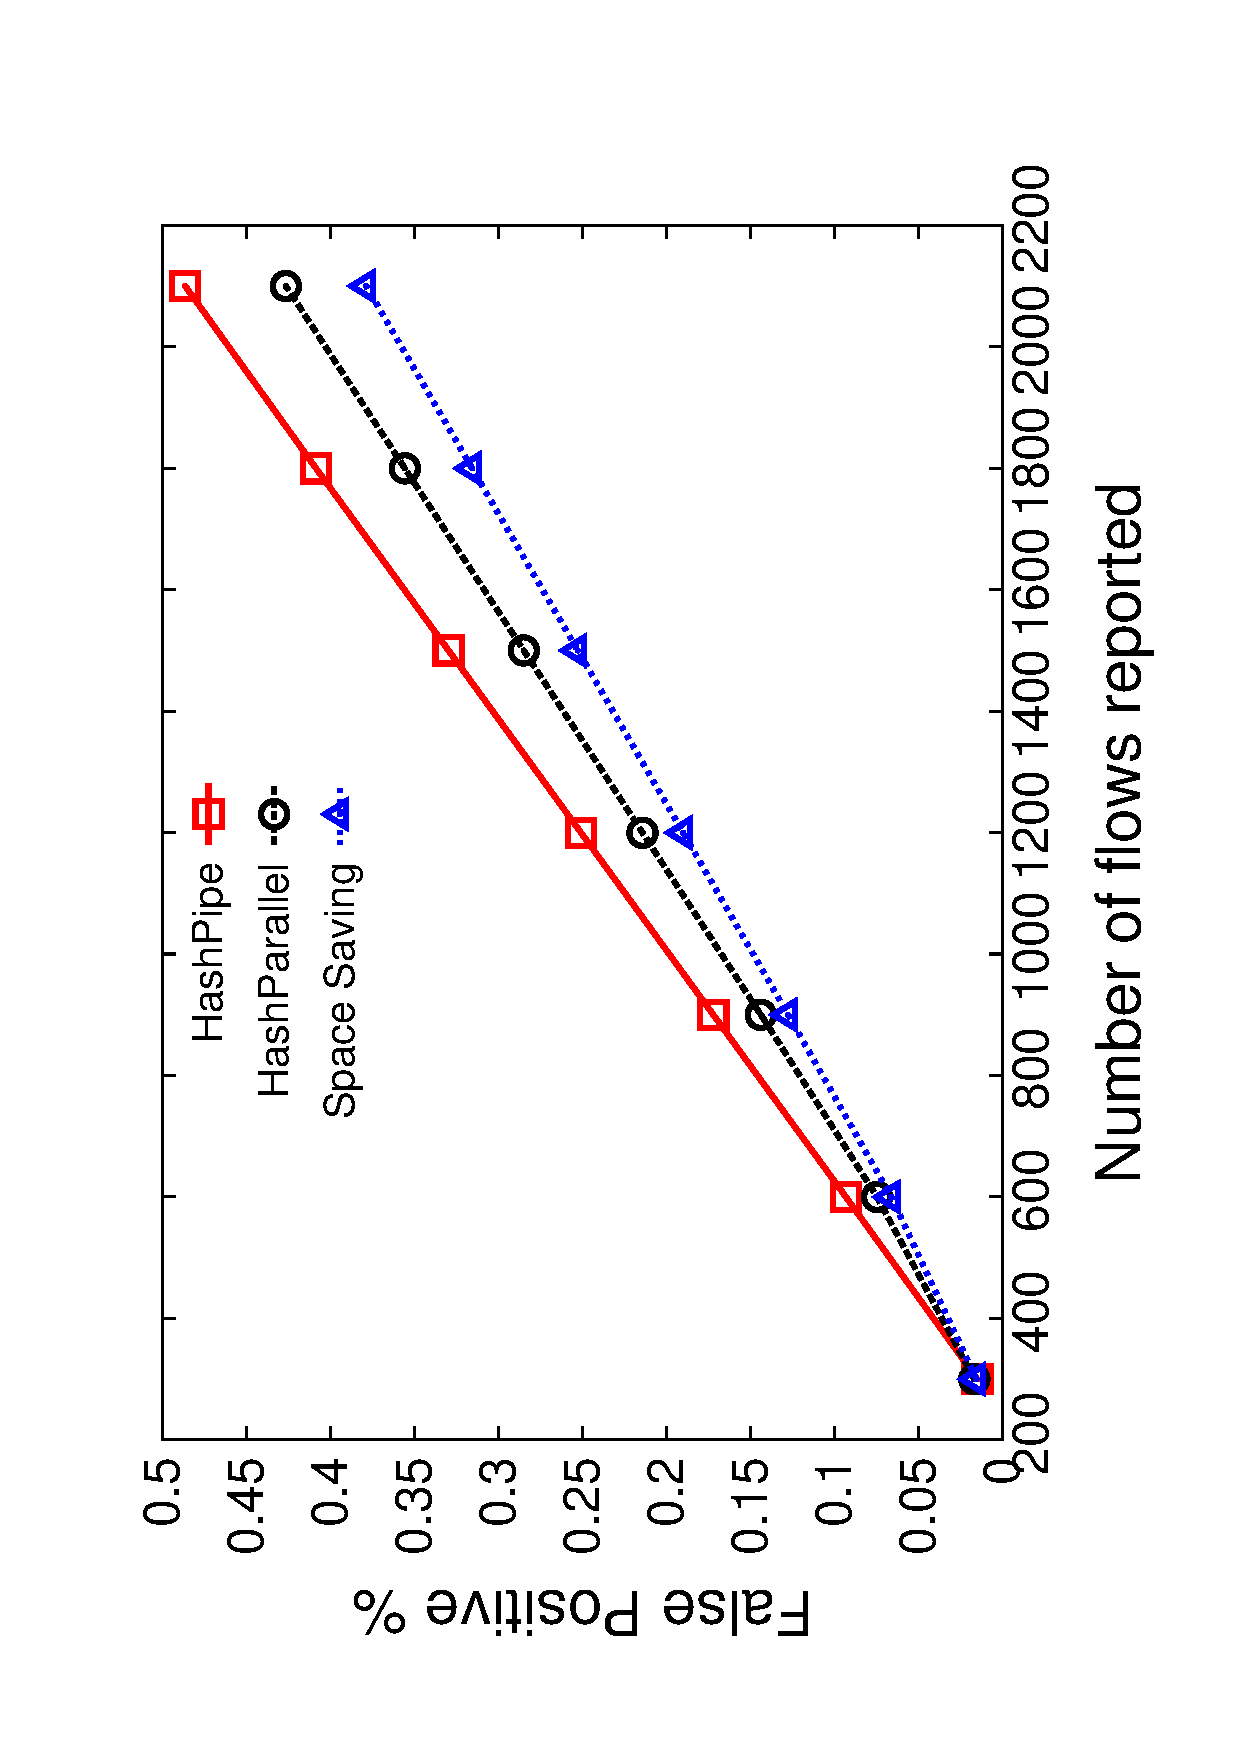
\includegraphics[width=0.95\columnwidth,max height=11cm,max width=8cm]{FriendsFalsePosWithRep.pdf}
\caption{Impact of overreporting flows from the table on false positive errors
  with $k$=300 heavy flows and $m$=2400 flows. %%The errors stay within a small
  %%range.}
  }
\label{fig:reportingMoreThanK-falsepos}
\end{figure}
\fi

%%
%- scatter plots to show where errors arise in our scheme. Sources of error include effect of hash collisions and packet interleaving. Possibly talk about prevalence of duplicates in sequential probing as a source of error. (generate graph here)
%- impact of (i) subsampling the table (as opposed to looking at the entire table), assuming you see all $D$ probes at once (ii) partial knowledge/sequential lookup instead of seeing all $D$ locations at once.
%(the two categorizations above may lead to the same!)
%%

%%

%zoomed in only top 1000 flows
%Focusing on only the top 1000 flows
%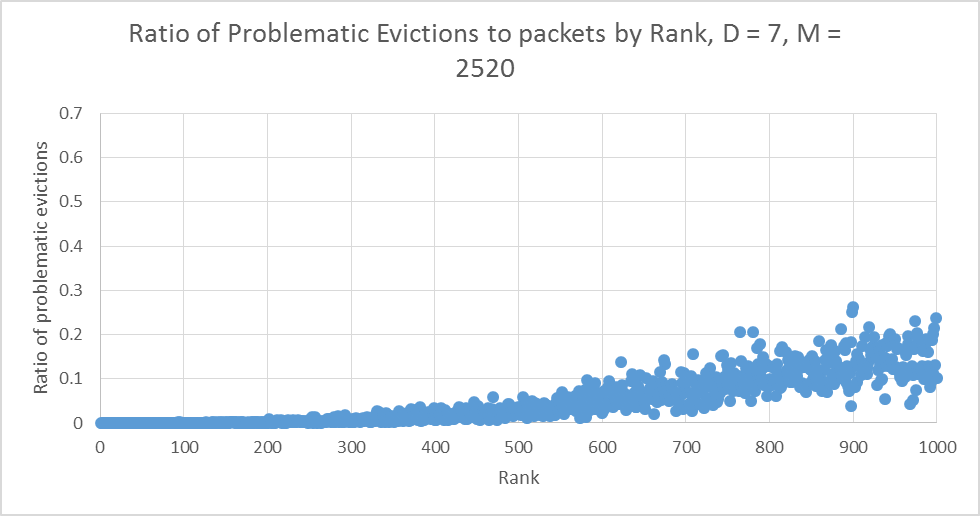
\includegraphics[max height=11cm,max width=8cm]{image031}
%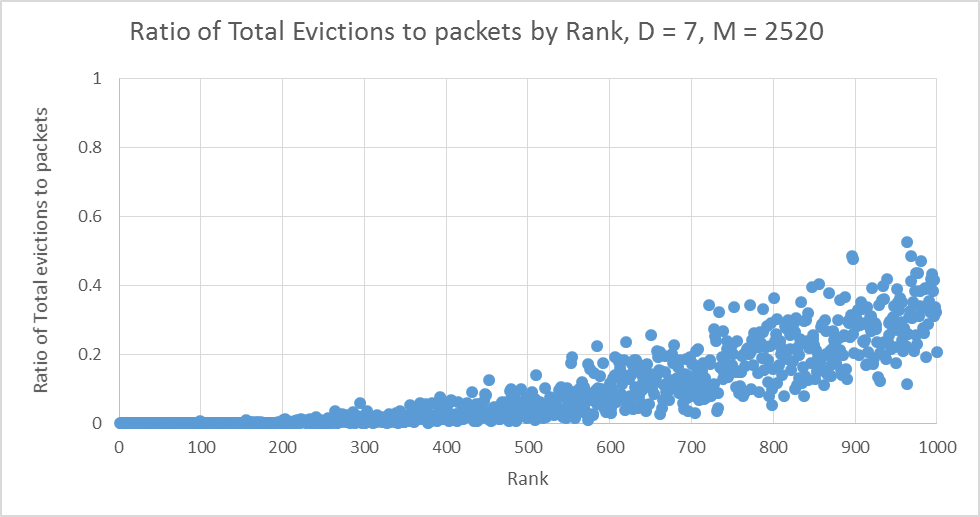
\includegraphics[max height=11cm,max width=8cm]{image033}


